%%%%%%%%%%%%%%%%%%%%%%%%%%%%%%%%%%%%%%%%%
% University/School Laboratory Report
% LaTeX Template
% Version 3.1 (25/3/14)
%
% This template has been downloaded from:
% http://www.LaTeXTemplates.com
%
% Original author:
% Linux and Unix Users Group at Virginia Tech Wiki 
% (https://vtluug.org/wiki/Example_LaTeX_chem_lab_report)
%
% License:
% CC BY-NC-SA 3.0 (http://creativecommons.org/licenses/by-nc-sa/3.0/)
%
%%%%%%%%%%%%%%%%%%%%%%%%%%%%%%%%%%%%%%%%%

%----------------------------------------------------------------------------------------
%	PACKAGES AND DOCUMENT CONFIGURATIONS
%----------------------------------------------------------------------------------------

\documentclass{article}

\usepackage[version=3]{mhchem} % Package for chemical equation typesetting
\usepackage{siunitx} % Provides the \SI{}{} and \si{} command for typesetting SI units
\usepackage{graphicx} % Required for the inclusion of images
\usepackage{natbib} % Required to change bibliography style to APA
\usepackage{amsmath} % Required for some math elements 
\usepackage[utf8]{inputenc}
\usepackage{tikz,pgfplots}
\usepackage[letterpaper, margin=0.5in]{geometry}
\usepackage{float}
\usepackage{enumitem}
\usepackage{gensymb}
\usepackage[hidelinks,bookmarks]{hyperref}
\usepackage[all]{hypcap}
\usepackage{subfloat}
\usepackage{color}
\usepackage{listings}

% Roman numerials
\pagenumbering{arabic}

\setlength\parindent{0pt} % Removes all indentation from paragraphs

%\renewcommand{\labelenumi}{\alph{enumi}.} % Make numbering in the enumerate environment by letter rather than number (e.g. section 6)

%\usepackage{times} % Uncomment to use the Times New Roman font

% for some tables
\newcommand{\specialcell}[2][c]{%
  \begin{tabular}[#1]{@{}c@{}}#2\end{tabular}}
  
\newcommand{\me}{\mathrm{e}}
\providecommand{\e}[1]{\ensuremath{\times 10^{#1}}}

\newcommand{\eqname}[1]{\tag*{#1}}

\renewcommand{\labelitemii}{$\circ$}

\DeclareMathOperator\erfc{erfc}

%%%%%%%%%%%% COLOR DEFINITIONS %%%%%%%%%%%%%

\definecolor{silicon}{RGB}{255,102,102}
\definecolor{oxide}{RGB}{145,150,110}
\definecolor{ioxide}{RGB}{175,180,135}
\definecolor{goxide}{RGB}{195,200,150}
\definecolor{poly}{RGB}{155,20,155}
\definecolor{spinglass}{RGB}{200,205,100}
\definecolor{n+}{RGB}{250,15,15}
\definecolor{aluminum}{RGB}{30,30,30}

%----------------------------------------------------------------------------------------
%	DOCUMENT INFORMATION
%----------------------------------------------------------------------------------------

%\title{Determination of the Atomic \\ Weight of Magnesium \\ CHEM 101} % Title

%\author{John \textsc{Smith}} % Author name

%\date{\today} % Date for the report

\begin{document}

%\maketitle % Insert the title, author and date

% If you wish to include an abstract, uncomment the lines below
% \begin{abstract}
% Abstract text
% \end{abstract}

%----------------------------------------------------------------------------------------
%	SECTION 1
%----------------------------------------------------------------------------------------

\section{Measurements \& Parameter Extraction}

\subsection{Line Width/Misalignment}

\subsubsection{Measured line widths}
\begin{figure}[H]
\centering
\begin{tabular}{c || c | c | c | c}
\specialcell{Nominal \\ Linewidth} & \specialcell{ACTV \\ (dark field)} & \specialcell{POLY \\ (clear field)} & \specialcell{CONT \\ (dark field)} & \specialcell{METAL \\ (clear field)} \\ \hline
2$\mu$m & 3 & 4 & 1.869 & 2.520 \\ \hline
\end{tabular}
\end{figure}

\subsubsection{Misalignment}

\subsection{Four-Point Resistors [2a, 2b]} %%%%%%%%%%%%% Resistors 2a 2b

\subsubsection{Measurement Setup}
\begin{figure}[H]
\centering
\begin{tikzpicture}
\node at (5,5) {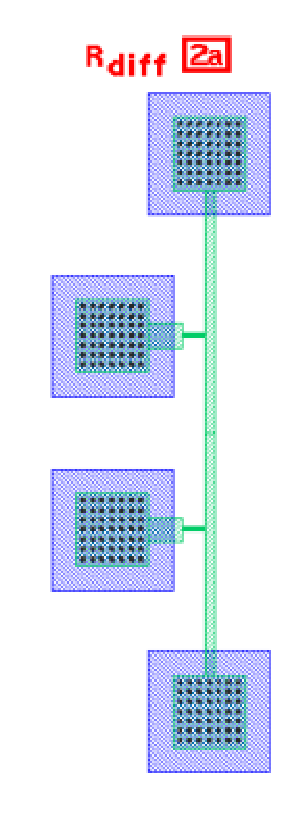
\includegraphics[height=250pt]{Device_setup/device2a1.pdf}};
\draw [<->,thick] (6,7.8) -- (8,7.8) -- (8,7.5); %SIM4
\node at (10,7.3) {I sweep, -0.1 to 0.1 A, comp 5, I measured};
\draw [<->,thick] (6,1.8) -- (8,1.8) -- (8,2.2); %Sim3
\node at (8,2.35) {GND};
\draw [<->,thick] (5,5.5) -- (7,5.5); %SIM1
\node at (9.5,5.5) {GND, comp 5, measure V};
\draw[<->,thick] (5,4) -- (7,4); %SIM2
\node at (9.5,4) {GND, comp 5, measure V};
\node at (15,5) {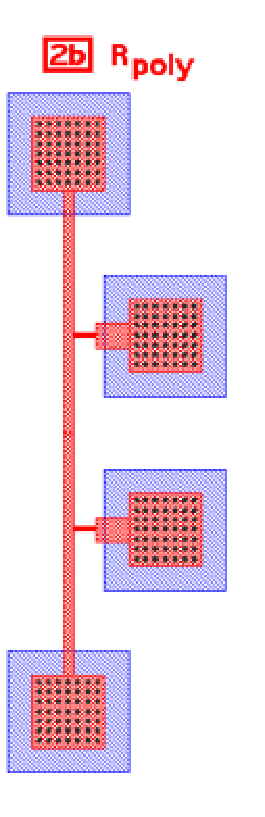
\includegraphics[height=250pt]{Device_setup/device2b1.pdf}};
\draw [<->,thick] (14,7.8) -- (8,7.8) -- (8,7.5); %SIM4
\draw [<->,thick] (14,1.8) -- (8,1.8) -- (8,2.2); %Sim3
\draw [<->,thick] (15,5.5) -- (12,5.5); %SIM1
\draw[<->,thick] (15,4) -- (12,4); %SIM2
\node at (5.2,7.8) {\textbf{A}};
\node at (4,4.7) {\textbf{VDiff}};
\draw[->,thick] (4.1,4.8) -- (4.2,5.1);
\draw[->,thick] (4.1,4.6) -- (4.2,4.4);
\end{tikzpicture}
\caption{Device 2a is a diffusion resistor and 2b is a poly resistor.}
\end{figure}

\subsubsection{I-V plot for the diffusion resistor, 2a}
\begin{figure}[H]
\centering
\begin{tikzpicture}
\node at (5,5) {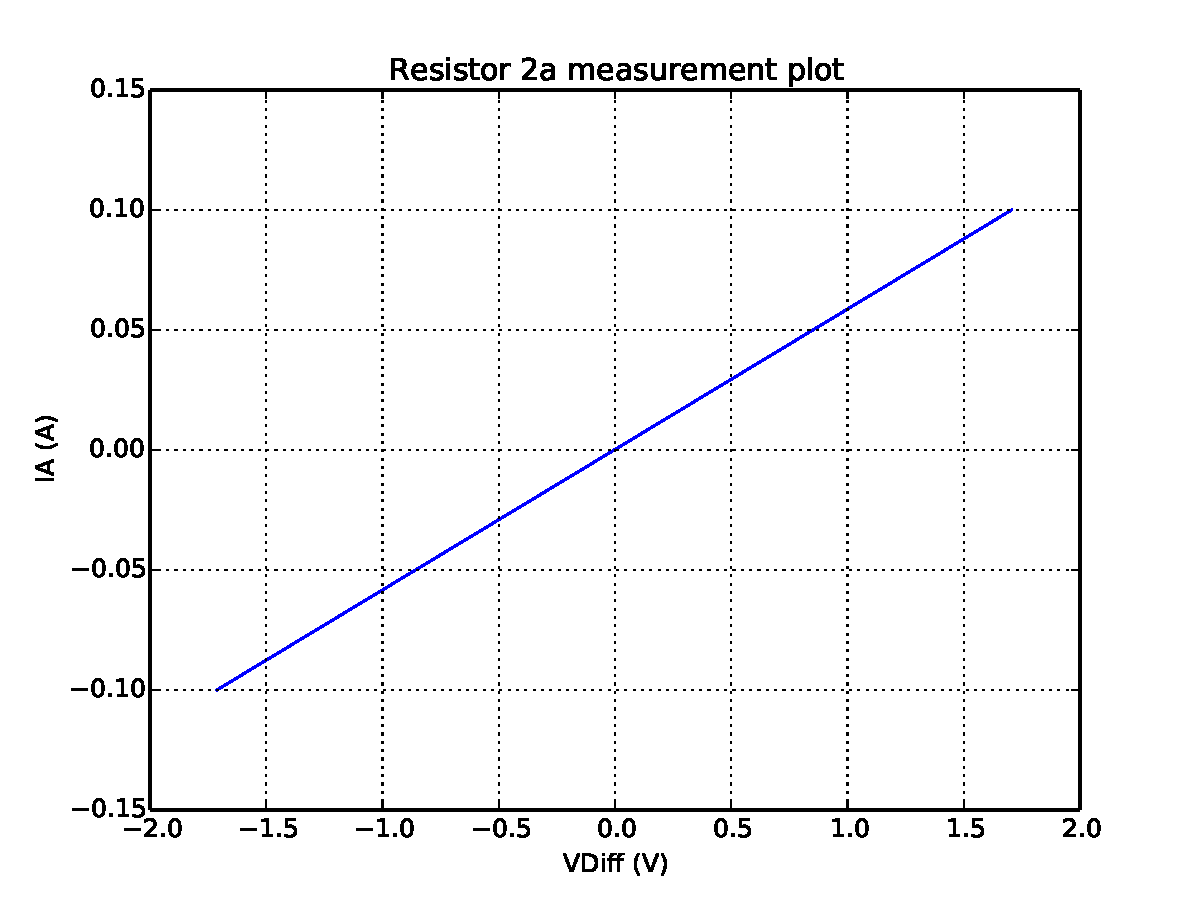
\includegraphics[width=250pt]{Device_plot_data/D2aplot.pdf}};
\end{tikzpicture}
\caption{A plot of the measurement data taken for resistor 2a. The plot is based off of 2 data points.}
\end{figure}

From the plot above we can calculate our resistance. Note that the slope of the above plot will be equal to 1/R. Since I = V/R, where I is our dependent variable (y axis) and V is our independent variable (X axis). A resistance of $R = 17 \,\Omega$ was calculated. Our width and length values are $10 \mu m$ and $200 \mu m$. However our final 2$\mu m$ line after the ACTV mask was 3 $\mu m$ which means that we had a overetch of about 50\%. This means that
\begin{align*}
R_s = \frac{W}{L}R_{\text{diff}} = \frac{10(1.50)}{200}17 = 1.28 \,\Omega
\end{align*}
From the previous lab report we have a junction depth of $1\,\mu m$. This means that our Resistivity is $\rho = R_s x_j = 1.07\e{-4}$ $\Omega$-cm. Using the Irvin curves in Jaeger [1], we can estimate the surface concentration $N_0 \approx 10^{21}$. Now the mobility can be calculated using a table of values from Appendix xx.
\begin{align*}
\mu_e = \mu_{\text{min}} + \frac{\mu_0}{1 + (N/N_{\text{ref}})^{\alpha}} = 92 + \frac{1268}{1 + (10^{21}/1.3\e{17})^{0.91}} = 92.4 \,\text{cm}^2 /V-s
\end{align*}

\subsubsection{I-V plot for the poly resistor, 2b}
\begin{figure}[H]
\centering
\begin{tikzpicture}
\node at (5,5) {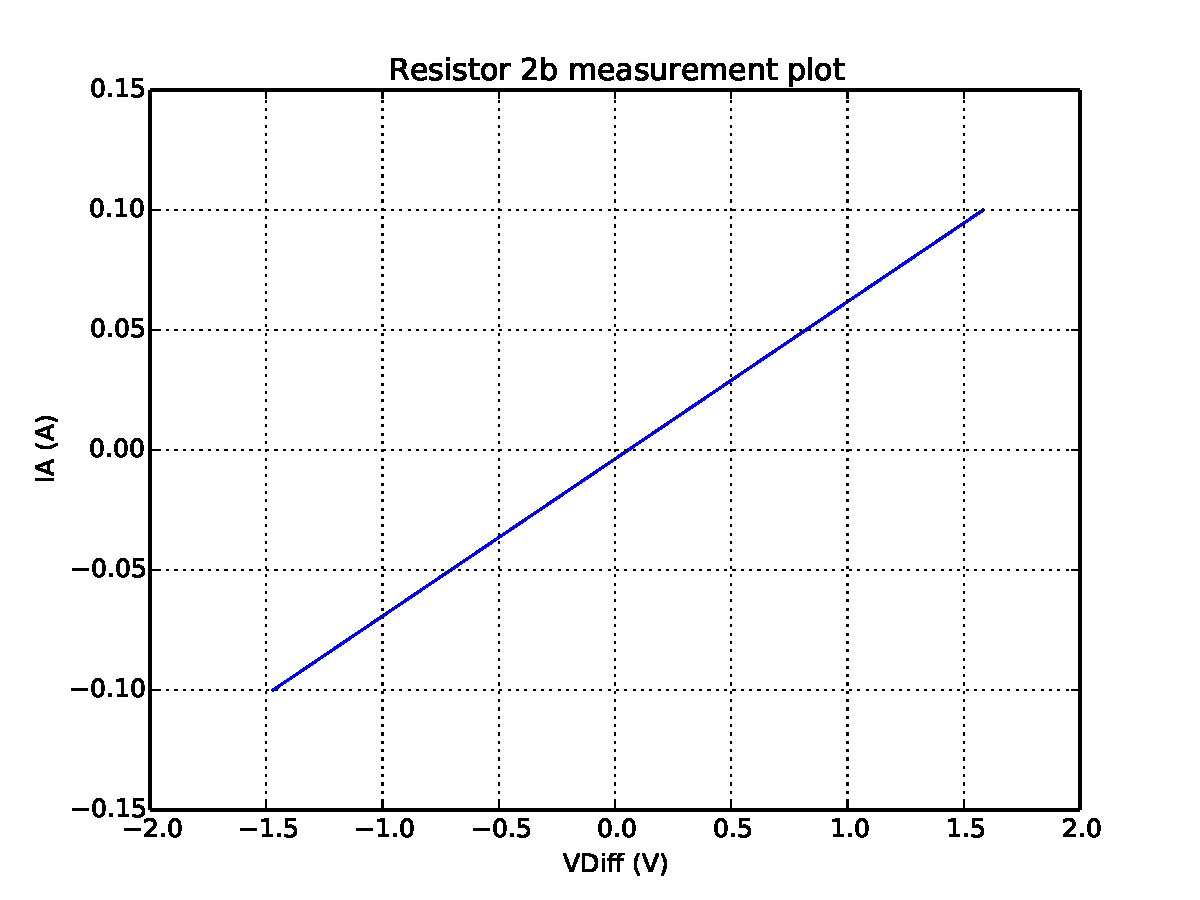
\includegraphics[width=250pt]{Device_plot_data/D2bplot.pdf}};
\end{tikzpicture}
\caption{A plot of the measurement data taken for resistor 2b. The plot is based off of 2 data points.}
\end{figure}

From the plot above we calculate a 1/slope value of 15. Hense $R = 15 \,\Omega$. This means that 
\begin{align*}
R_s = \frac{W}{L}R_{\text{poly}} = \frac{10(1.26)}{200}15 = 0.945 \,\Omega 
\end{align*}
Our Resistivity is then $\rho = R_s t_{\text{poly}}$ where $t_{\text{poly}}$ is the polysilicon thickness which is 0.4 $\mu m$, Hense $\rho = 0.378 \,\Omega$-$\mu m$.

\subsection{Four-Point Contact Resistor [17a, 17b]} %%%%%%%%%%%% Resistors 17a,b
\subsubsection{Measurement Setup}
\begin{figure}[H]
\centering
\begin{tikzpicture}
\node at (5,5) {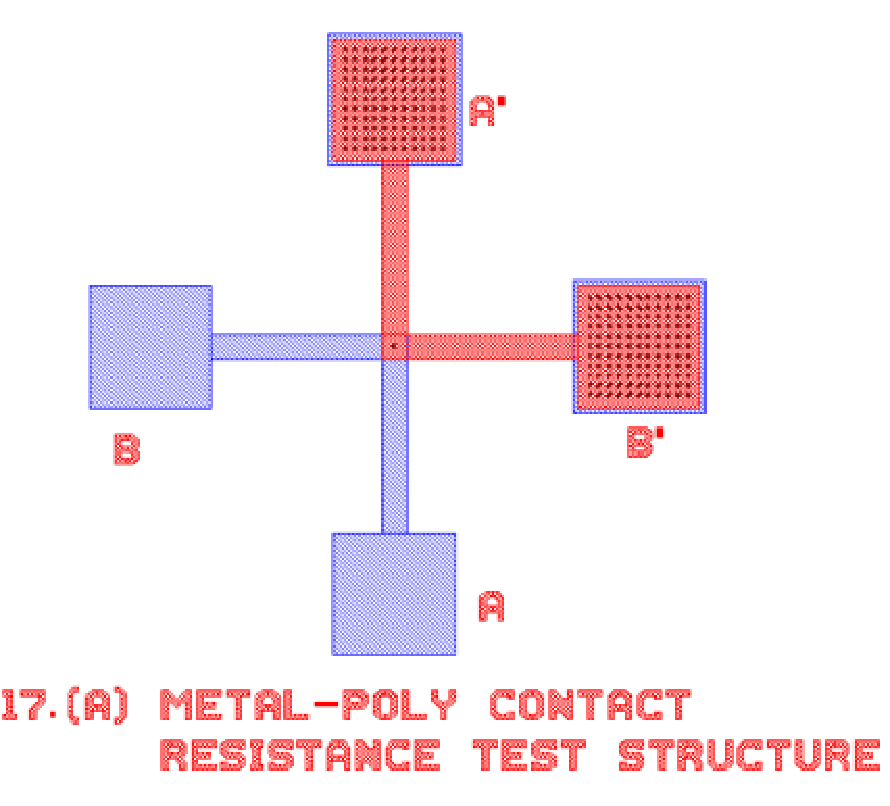
\includegraphics[width=250pt]{Device_setup/device17a2.pdf}};
\draw [<->] (4.5,8) -- (6,9); %Current sweep
\node at (6,9.2) {I sweep, -0.1 to 0.1 A, comp 5, measure I};
\draw [<->] (2,5.5) -- (2,6.5); %voltage
\node at (2,6.7) {V, constant};
\draw [<->] (7,5.5) -- (7,6.5); % const current
\node at (7,6.7) {I, constant, comp 5};
\draw [<->] (4.5,3) -- (3,3.8); % const current
\node at (2.5,4.1) {I, constant, comp 5};
\end{tikzpicture}
\caption{Measurement setup for 17a poly contact resistor. The same setup is used for the diffusion contact resistor, 17b.}
\end{figure}

\subsubsection{I-V plot for 17a, poly reisistor}
\begin{figure}[H]
\centering
\begin{tikzpicture}
\node at (5,5) {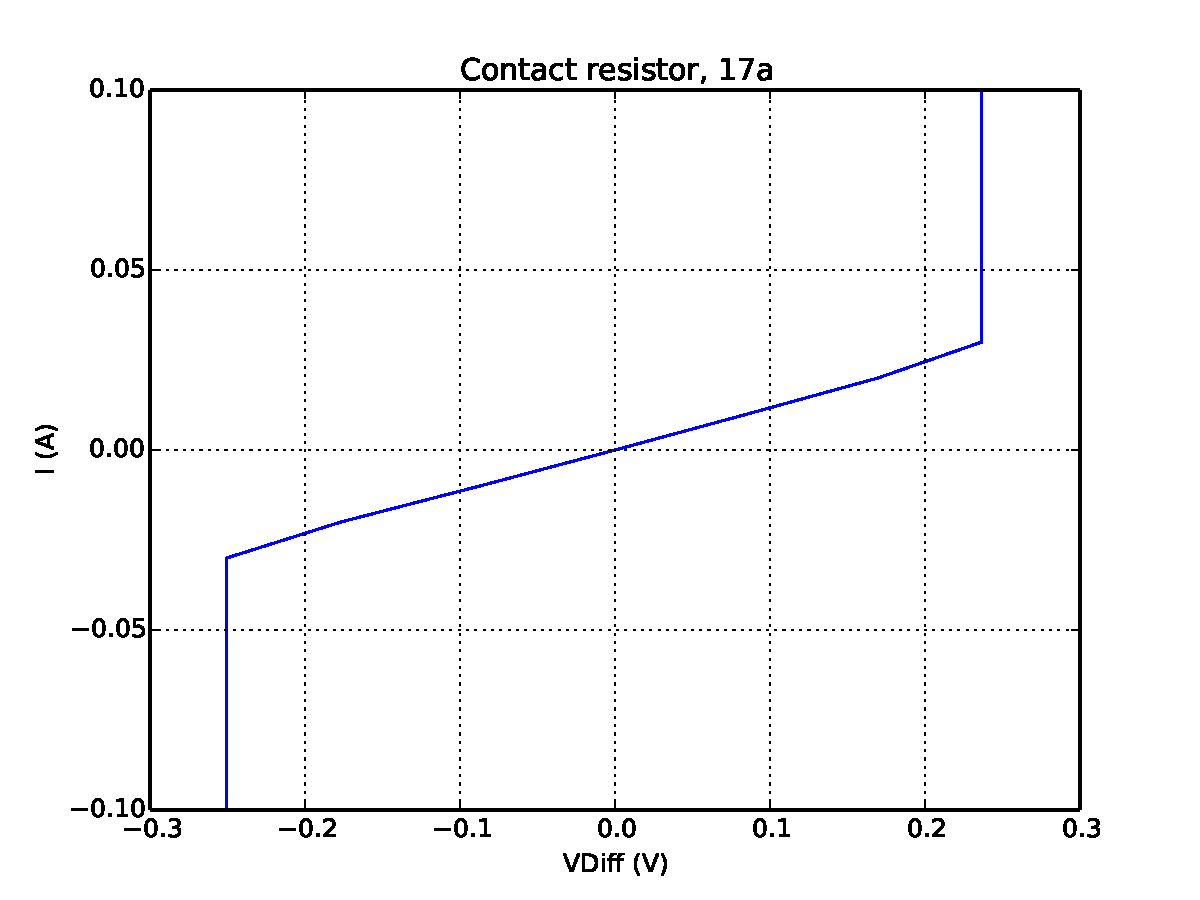
\includegraphics[width=250pt]{Device_plot_data/D17aplot.pdf}};
\end{tikzpicture}
\caption{A plot of the measurement data taken for resistor 17a.}
\end{figure}

From the above plot we calculated a resistance of $R = 8.54 \Omega$. Note that the slope above gives us $1/R$ so we need to take the inverse to find the resistance.

\subsubsection{I-V plot for 17b, diffusion resistor}
\begin{figure}[H]
\centering
\begin{tikzpicture}
\node at (5,5) {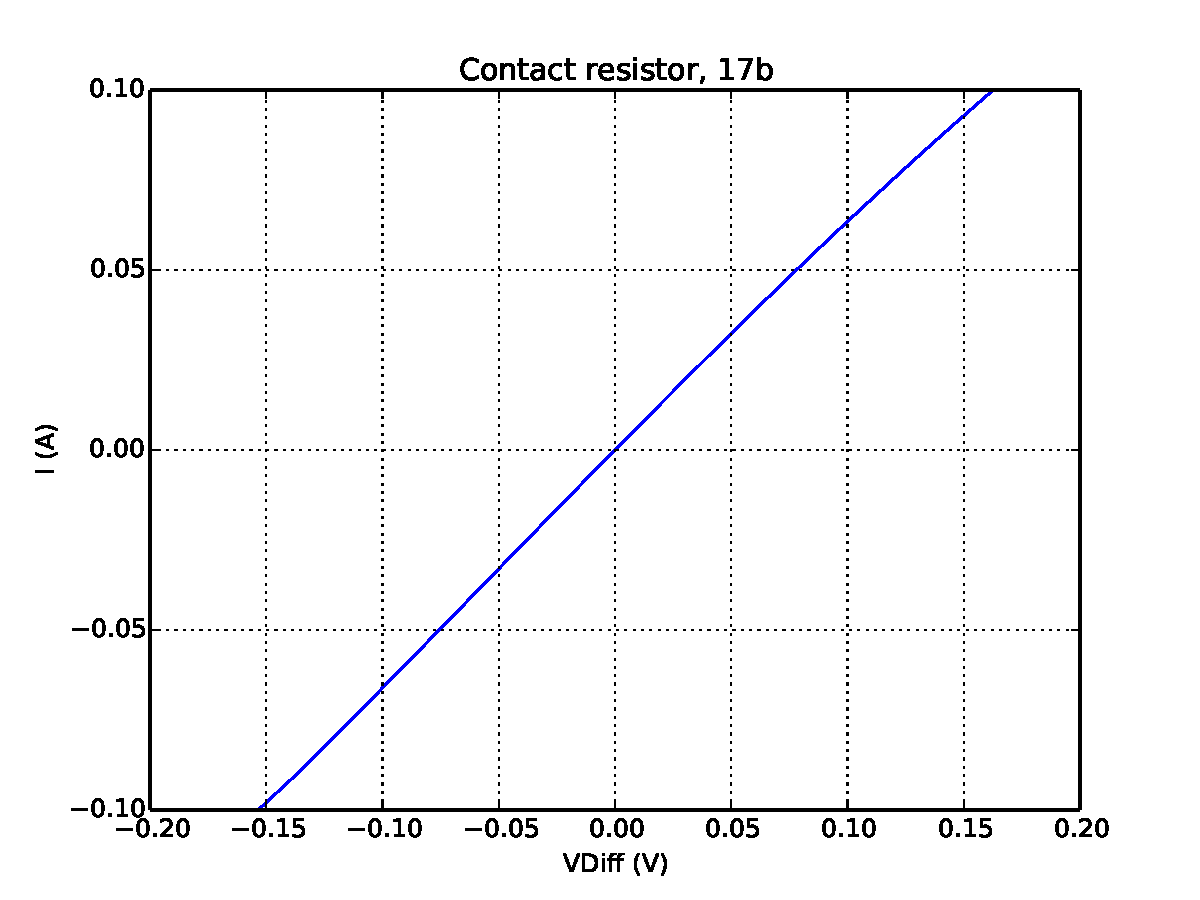
\includegraphics[width=250pt]{Device_plot_data/D17bplot.pdf}};
\end{tikzpicture}
\caption{A plot of the measurement data taken for resistor 17b.}
\end{figure}

Similarly, from the above plot we calculated a resistance of $R = 1.46 \Omega$.

\subsection{Four-Point Contact-Chain Resistor [2c, 2d]} %%%%%%%% Resistors 2c 2d

\subsubsection{Measurement Setup}
\begin{figure}[H]
\centering
\begin{tikzpicture}
\node at (5,5) {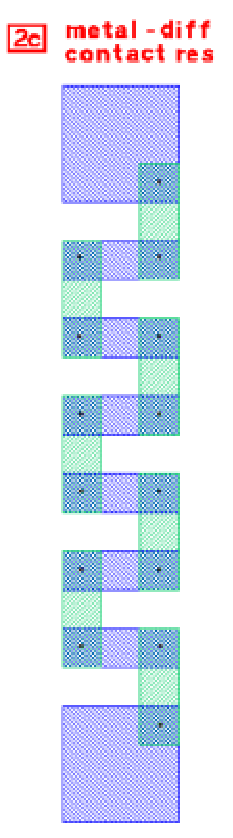
\includegraphics[height=250pt]{Device_setup/device2c2.pdf}};
\draw[<->,thick] (5,8) -- (8,8) -- (8,7); %Sim1
\node at (9,6.8) {V sweep, -5 to 5 V, measure I, V };
\draw[<->,thick] (5,1.5) -- (8,1.5) -- (8,2.5); %Sim2
\node at (8,3) {GND};
\node at (13,5) {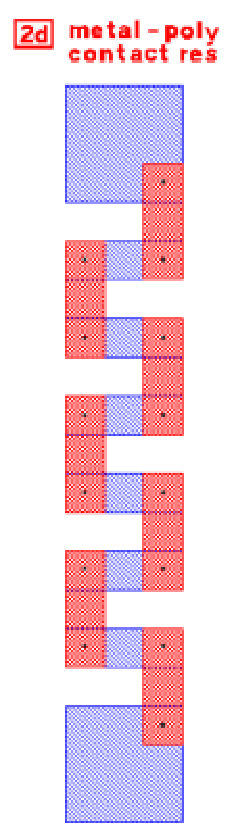
\includegraphics[height=250pt]{Device_setup/device2d2.pdf}};
\draw[<->,thick] (13,8) -- (8,8) -- (8,7); %Sim1
\draw[<->,thick] (13,1.5) -- (8,1.5) -- (8,2.5); %Sim2
\node at (4.8,8) {\textbf{A}};
\end{tikzpicture}
\caption{Chain resistor setup for diffusion and poly resistors.}
\end{figure}

\subsubsection{b. I-V plot for diffusion resistor, 2c}
\begin{figure}[H]
\centering
\begin{tikzpicture}
\node at (5,5) {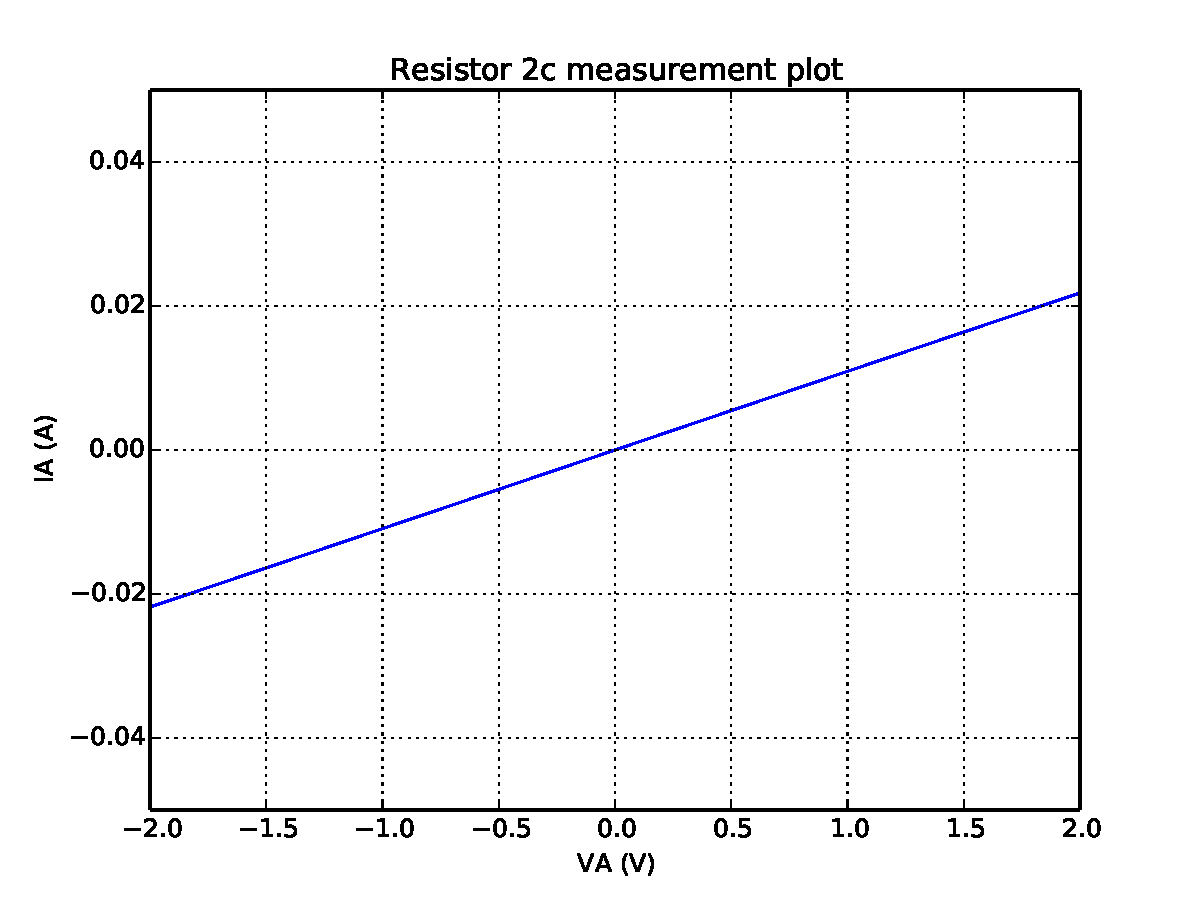
\includegraphics[width=250pt]{Device_plot_data/D2cplot.pdf}};
\end{tikzpicture}
\caption{A plot of the measurement data taken for resistor 2c. The plot is based off of 2 data points.}
\end{figure}

The resistance calculated from the graph here is $R = 91.2 \Omega$. Using sheet resistance from 2a/b and the total resistance from the slope above, we can solve for the contact resistance

\begin{align*}
R_{\text{total diff}} = 7(\eta R_{\text{S diff}} + R_{\text{C diff}}) \Rightarrow R_{\text{C diff}} = \frac{1}{7}R_{\text{total diff}} - \eta R_{\text{S diff}} = \frac{1}{7}(91.2 \Omega) - 2.3(1.07 \Omega) = 10.6 \Omega
\end{align*}



\subsubsection{b. I-V plot for poly resistor, 2d}
\begin{figure}[H]
\centering
\begin{tikzpicture}
\node at (5,5) {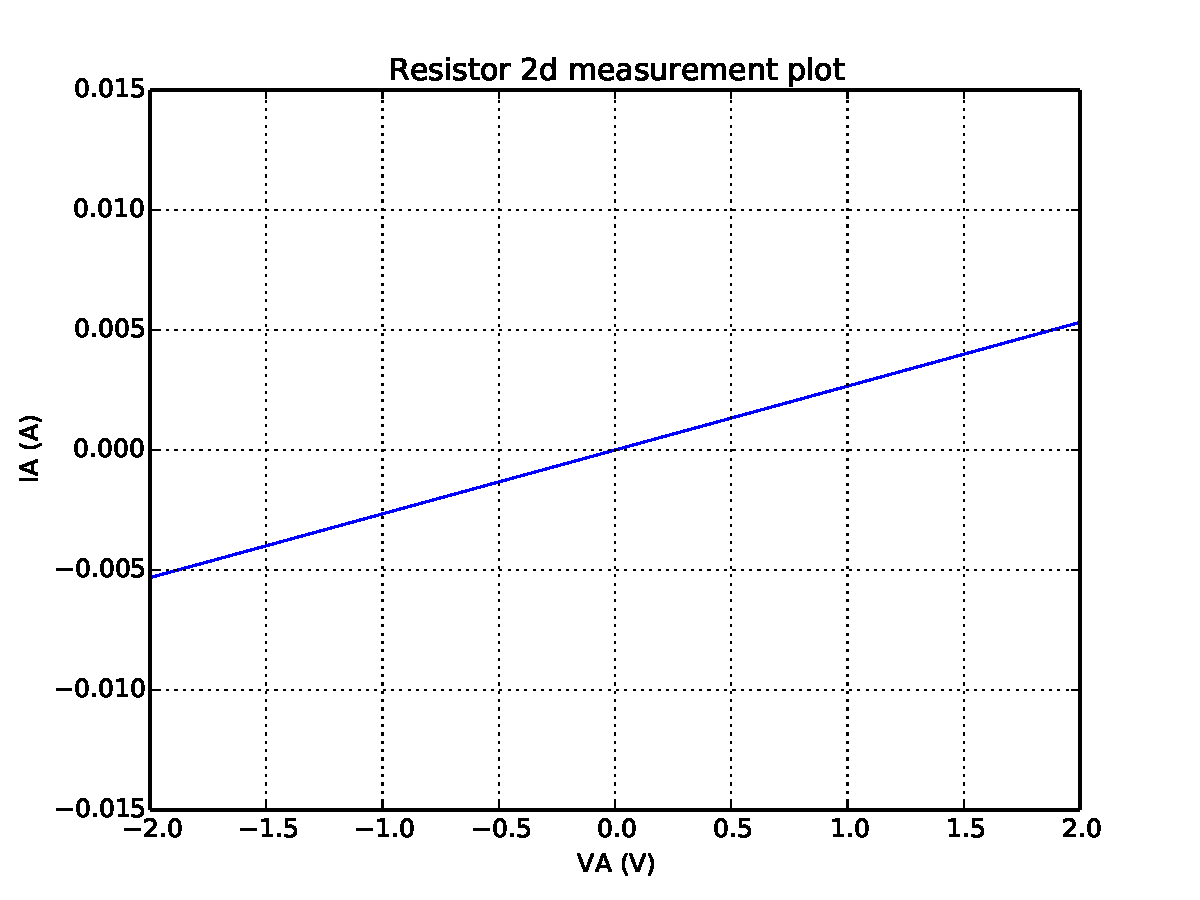
\includegraphics[width=250pt]{Device_plot_data/D2dplot.pdf}};
\end{tikzpicture}
\caption{A plot of the measurement data taken for resistor 2d. The plot is based off of 2 data points.}
\end{figure}

The resistance calculated from the graph here is $R = 370 \Omega$. Using sheet resistance from 2a/b and the total resistance from the slope above, we can solve for the contact resistance

\begin{align*}
R_{\text{total poly}} = 7(\eta R_{\text{S poly}} + R_{\text{C poly}}) \Rightarrow R_{\text{C poly}} = \frac{1}{7}R_{\text{total poly}} - \eta R_{\text{S poly}} = \frac{1}{7}(370 \Omega) - 2.3(0.945 \Omega) = 50.7 \Omega
\end{align*}


\subsection{Gate Oxide Capacitor, 4} %%%%%%% Gate capacitor 4

\subsubsection{Measurement Setup}
\begin{figure}[H]
\centering
\begin{tikzpicture}
\node at (5,5) {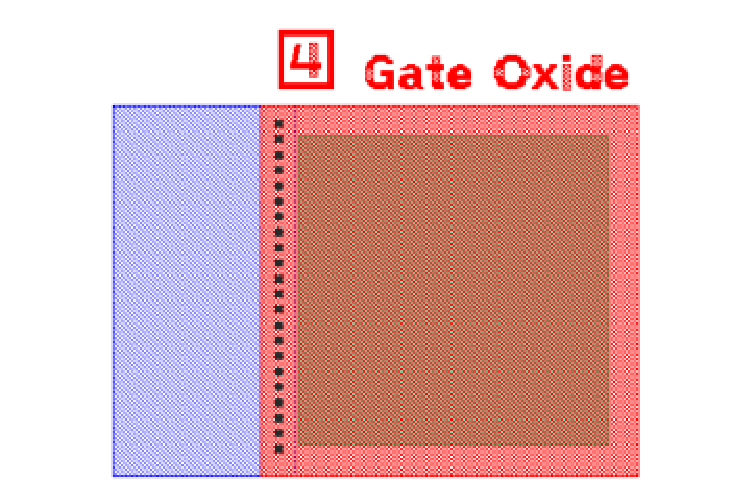
\includegraphics[width=250pt]{Device_setup/device4a2.pdf}};
\node at (5,8) {Stage connector set to GND};
\node at (3,5) {\textbf{A}};
\draw[<->,thick] (3,4) -- (3,2.2);
\node at (5,2){V sweep, -10 to 10 V, step 0.2 V, oscillation 0.02Hz, integration medium};
\end{tikzpicture}
\caption{Gate capacitor setup.}
\end{figure}


\subsubsection{C-V plot of gate oxide capacitor w/ lights ON}
\begin{figure}[H]
\centering
\begin{tikzpicture}
\node at (5,5) {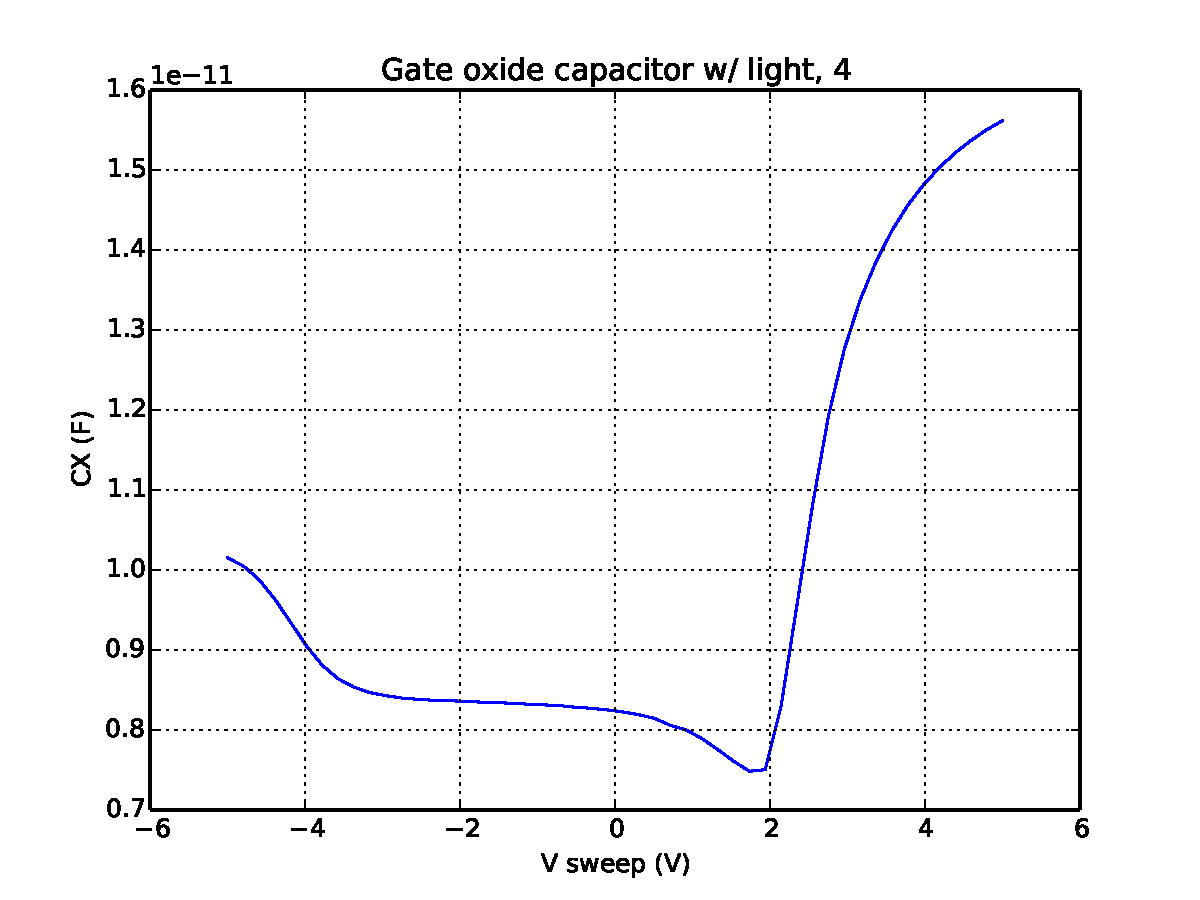
\includegraphics[width=250pt]{Device_plot_data/D4aplot.pdf}};
\end{tikzpicture}
\caption{A plot of the measurement data taken for the gate capacitor, 4. Lights on.}
\end{figure}

The minimum capacitance from the plot above is 7.48 pF. The accumulation region capacitance at about 5 V is 15.7 pF. The active area is 200 $\mu m$ by 200 $\mu m$ while the pad+ring area is 240 $\mu m$ by 335 $\mu m$. Also note the gate oxide thickness calculated below for the field oxide capacitors is 1.15 $\mu$m.

\subsubsection{C-V plot of gate oxide capacitor w/ lights OFF}
\begin{figure}[H]
\centering
\begin{tikzpicture}
\node at (5,5) {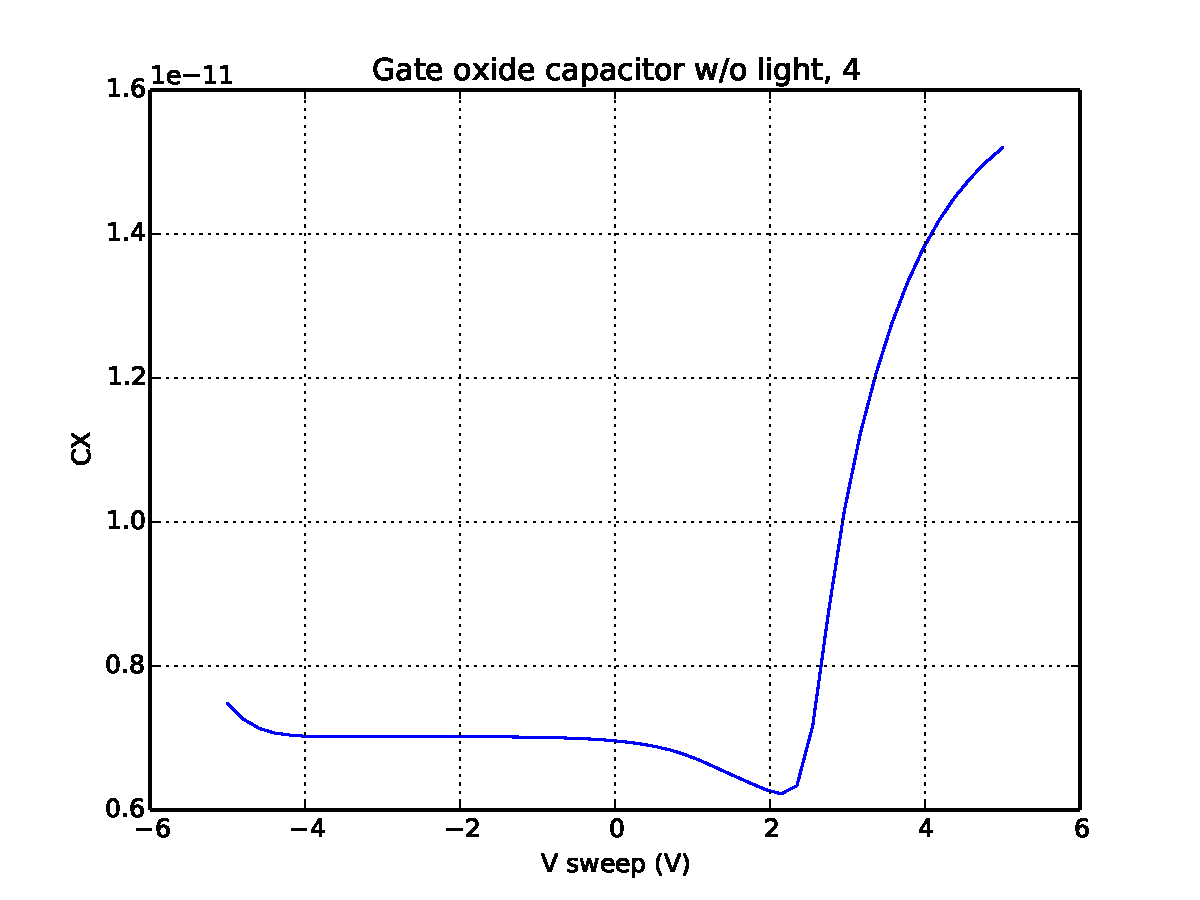
\includegraphics[width=250pt]{Device_plot_data/D4bplot.pdf}};
\end{tikzpicture}
\caption{A plot of the measurement data taken for the gate capacitor, 4. Lights off.}
\end{figure}

The minimum capacitance from the plot above is 6.22 pF. The accumulation region capacitance at about 5 V is 15.7 pF. The active area is 200 $\mu m$ by 200 $\mu m$ while the pad+ring area is 240 $\mu m$ by 335 $\mu m$. Also note the gate oxide thickness calculated below for the field oxide capacitors is 1.15 $\mu$m.

\begin{align*}
C_{\text{measured}} &= A_{\text{active}}\frac{\epsilon_{\text{ox}}}{t_{\text{gox}}} + A_{\text{pad-ring}}\frac{\epsilon_{\text{ox}}}{t_{\text{fox}}} \\ \\
t_{\text{gox}} = [\frac{1}{A_{\text{active}}}(\frac{C_{\text{measured}}}{\epsilon_{\text{ox}}} - \frac{A_{\text{pad-ring}}}{t_{\text{fox}}})]^{-1} &= [\frac{1}{4\e{-8}}(\frac{15.7\e{-12}}{(3.9)8.85\e{-12}} - \frac{8.04\e{-8}}{1.15\e{-6}})]^{-1} = 0.104 \,\mu\text{m}
\end{align*}
The capacitance per unit area in this case would be 15.7 pF / ($240 \mu m \times 335 \mu m$). C/area = 1.95 pF/$\mu$m or 1.95 F/$m^{-2}$. Now in order to calculate the maximum depletion region we use an equation from lecture notes. Note the max and min capacitance we calculated earlier,
\begin{equation}
\frac{1}{C_{\text{min}}} = \frac{1}{C_{\text{max}}} + \frac{1}{A_{\text{pad-ring}} C_{\text{Dmin}}},\,\text{where } C_{\text{Dmin}} = \frac{\epsilon_{\text{si}}}{x_{\text{dmax}}}
\end{equation}
Solving for the maximum depletion region we get,
\begin{align*}
x_{\text{dmax}} = A_{\text{pad-ring}}\epsilon_{\text{si}}(\frac{1}{C_{\text{min}}} - \frac{1}{C_{\text{max}}}) = (8.04\e{-8})(11.7 \times 8.85\e{-12})(\frac{1}{6.22\e{-12}} - \frac{1}{15.7\e{-12}}) = 0.808 \mu m
\end{align*}

Another equation from lecture will help us solve for the substrate doping concentration,
\begin{equation}
x_d = \sqrt{\frac{2\epsilon_{\text{si}}}{q}\frac{1}{N_A}|\psi_s|}
\end{equation}
where $\psi_s$ is the potential drop and has a typical value of 0.3, q is the charge of an electron 1.602\e{-19} C, and $N_A$ is the doping concentration.
\begin{align*}
N_A = \frac{2\epsilon_{\text{si}} |\psi_s|}{q{x_d}^2} = \frac{2(11.7 \times 8.85\e{-12})(0.3)}{1.602\e{-19}(0.808\e{-6})^2} = 5.94\e{20} \,{\text{m}}^{-3}
\end{align*}
From the curve above (Figure 11) we can see that the flatband voltage is $V_{FB} \approx 5.5$ and the corresponding $C_{FB} \approx 15.5$pF. To find the charge per unit area at the oxide silicon interface we can use the Q = CV equation.
\begin{align*}
\frac{Q_{ss}}{A} = \frac{C_{FB}V_{FB}}{A_{\text{pad-ring}}} = \frac{(5.5)(15.5\e{-12})}{8.04\e{-8}} = 1.06 \,\text{mF}/\text{m}^2
\end{align*}
To calculate the threshold voltage we will assume that $V_{SB} = 0$. First we must also calculate $Q_{BO}$ which is the charge stored in the depletion region,
\begin{align*}
Q_{BO} = \sqrt{2q\epsilon_{si}N_B2\phi_F} = \sqrt{2(1.602\e{-19})(11.7 \times 8.85\e{-12})(5.94\e{20})(2 \times 0.3)} = 1.09\e{-4}\, C/{\text{m}}^2
\end{align*}
Now to calculate/estimate threshold voltage. Note that the work function $\phi_{ms}$ is zero for n+ doped poly gate.
\begin{align*}
V_t = \phi_{ms} + 2\phi_f - \frac{Q_{ss}}{C_{\text{max/area}}} + \frac{Q_{BO}}{C_{\text{max/area}}} = 0 + 0.6 - \frac{1.06\e{-3}}{1.95} + \frac{1.09\e{-4}}{1.95} = 0.600 V
\end{align*}

\subsection{Field Oxide Capacitor, 3} %%%%%%% Field Oxide Capacitors 3

\subsubsection{Measurement Setup}
\begin{figure}[H]
\centering
\begin{tikzpicture}
\node at (5,5) {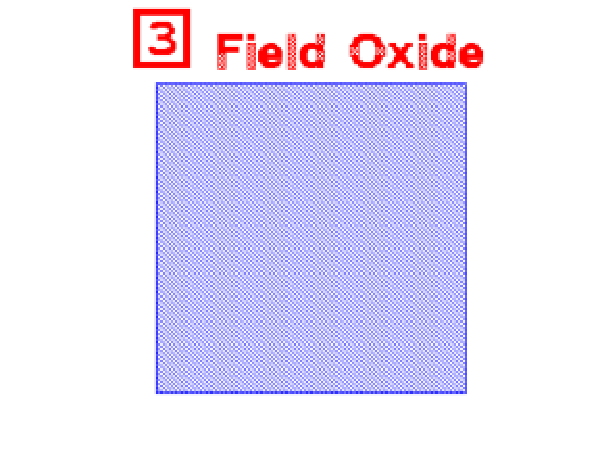
\includegraphics[width=250pt]{Device_setup/device3a2.pdf}};
\node at (5,9) {Stage connector set to GND};
\node at (5,5) {\textbf{A}};
\draw[<->,thick] (5,4) -- (5,2.2);
\node at (5,2){V sweep, -5 to 5 V, step 0.2 V, oscillation 0.02Hz, integration medium};
\end{tikzpicture}
\caption{Field oxide capacitor setup.}
\end{figure}


\subsubsection{C-V plot of field oxide capacitor}
\begin{figure}[H]
\centering
\begin{tikzpicture}
\node at (5,5) {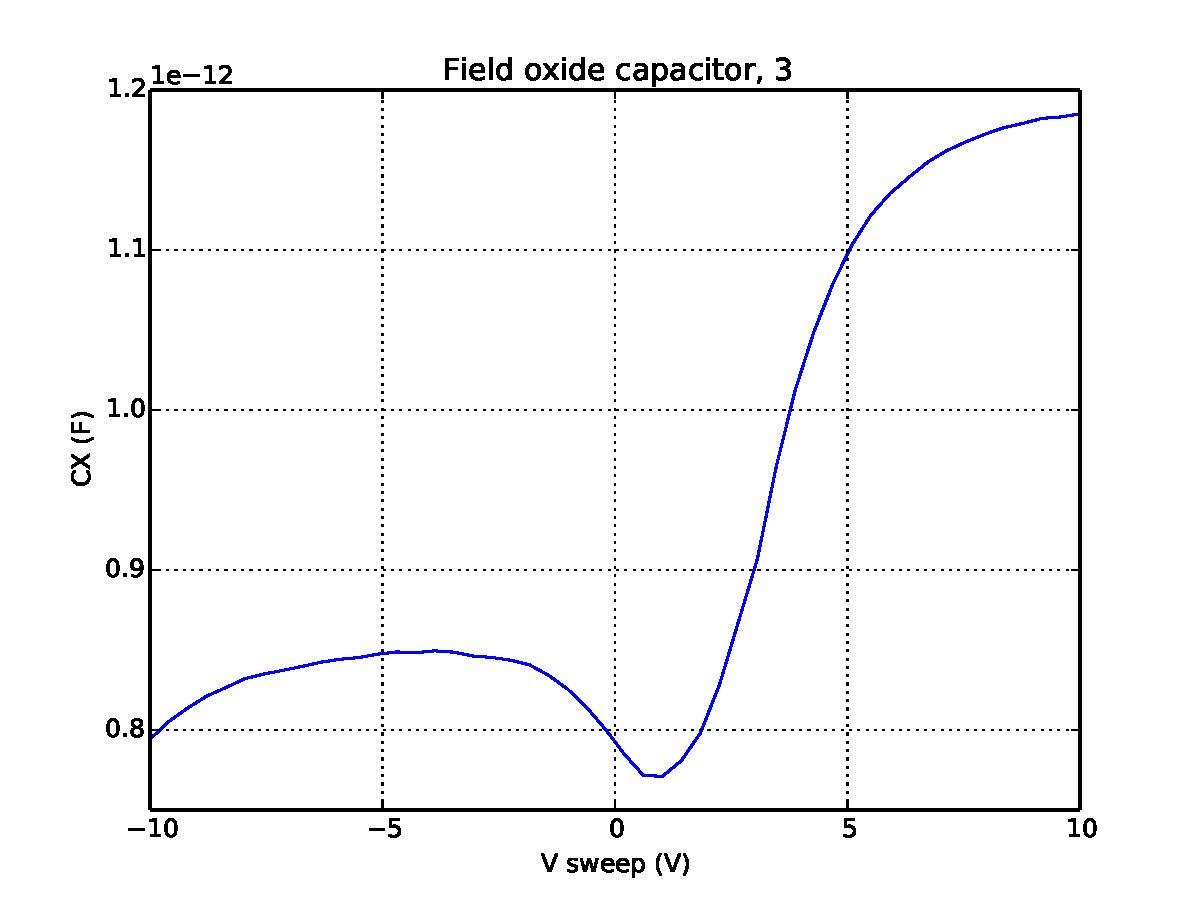
\includegraphics[width=250pt]{Device_plot_data/D3plot.pdf}};
\end{tikzpicture}
\caption{A plot of the measurement data taken for the field oxide capacitor, 3}
\end{figure}

From the plot above we see that at the accumulation region of $\approx 10$ volts we have a corresponding capacitance of $C \approx 1.2$pF. Noting that the area of the capacitor plate is 200 $\mu m$ by 200 $\mu m$, we can now solve for the dieletric (oxide) thickness.
\begin{align*}
C = \frac{A \epsilon_{\text{ox}}}{t_{\text{fox}}} \Rightarrow t_{\text{fox}} = \frac{3.9 A \epsilon_0}{C} = \frac{3.9 (4\e{-8}) (8.85\e{-12})}{1.2 \e{-12}} = 1.15 \,\mu\text{m}
\end{align*}

\subsection{Intermediate Oxide Capacitors, 5} %%%%%%% Intermediate Oxide Capacitor 5

\subsubsection{Measurement Setup}
\begin{figure}[H]
\centering
\begin{tikzpicture}
\node at (5,5) {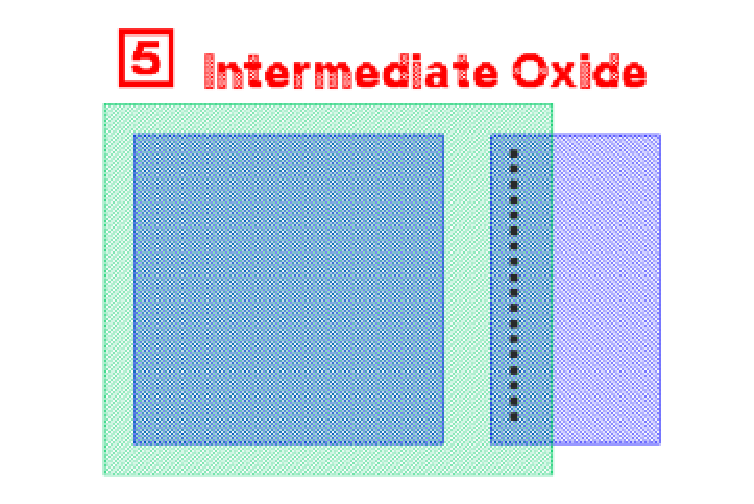
\includegraphics[width=250pt]{Device_setup/device5a2.pdf}};
\node at (5,5) {\textbf{A}};
\node at (7.5,5) {\textbf{K}};
\draw[<->,thick] (5,4) -- (5,2.2);
\node at (5,2){V sweep, -5 to 0 V, step 0.2 V, oscillation 0.02Hz, integration medium};
\draw[<->,thick] (7.5,4) -- (9,5);
\node at (9,5.2) {GND};
\end{tikzpicture}
\caption{Intermediate oxide capacitor setup.}
\end{figure}


\subsubsection{C-V plot of intermediate oxide capacitor}
\begin{figure}[H]
\centering
\begin{tikzpicture}
\node at (5,5) {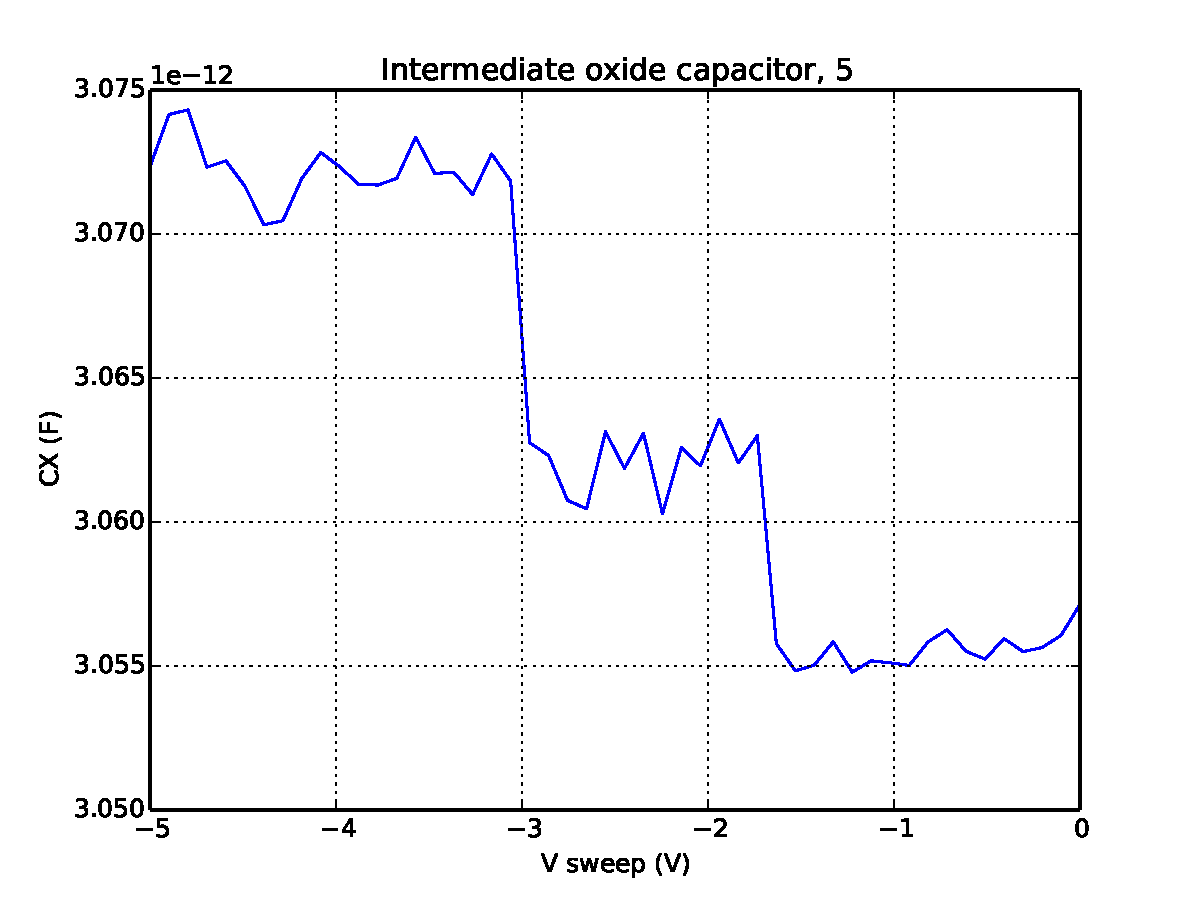
\includegraphics[width=250pt]{Device_plot_data/D5plot.pdf}};
\end{tikzpicture}
\caption{A plot of the measurement data taken for the Intermediate oxide, 5}
\end{figure}

The capacitance at the accumulation region of $\approx 5$ V is about 3.0725 pF.


\subsection{Diode, 7} %%%%%%%%% Diode 7

\subsubsection{Measurement setups for forward and reverse operations}
\begin{figure}[H]
\centering
\begin{tikzpicture}
\node at (5,5) {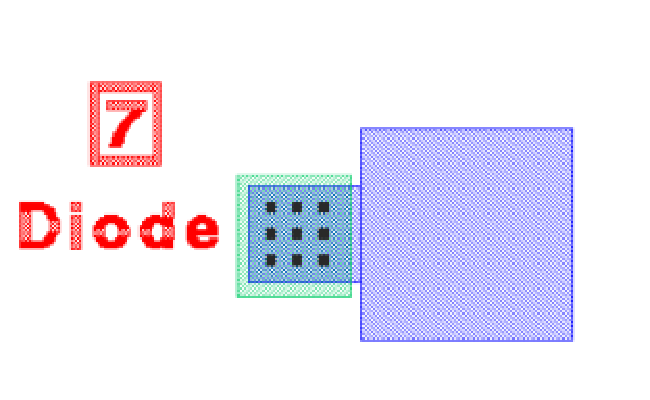
\includegraphics[width=200pt]{Device_setup/device7a2.pdf}};
\node at (15,5) {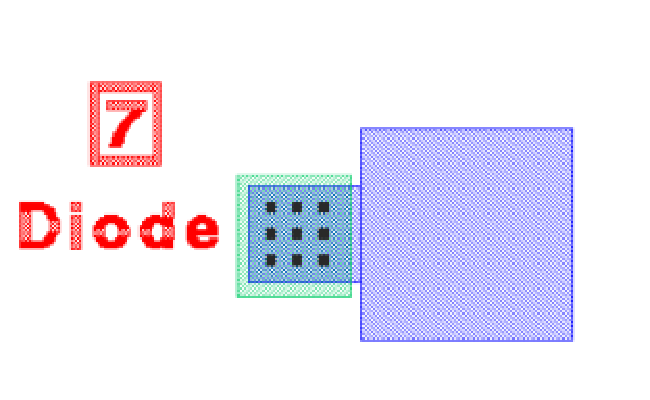
\includegraphics[width=200pt]{Device_setup/device7a2.pdf}};
\node at (6.5,4.5) {\textbf{A}};
\node at (16.5,4.5) {\textbf{A}};
\draw[<->,thick] (6,5) -- (9,5) -- (9,6);
\node at (9,6.2) {V sweep, -1 to 1 V, measure I, V };
\node at (5,3) {Stage connector set to GND};
\draw[<->,thick] (17,4.5) -- (17,3.6) -- (13,3.6) -- (13,3.2);
\node at (13,3.0) {V sweep, -40 to 40 V, comp 0.05, measure I, V };
\node at (13,2.5) {Stage connector set to -40 V, comp 0.05};
\node at (5,7) {\textbf{Test 1 (forward)}};
\node at (15,7) {\textbf{Test 2 (reverse)}};
\end{tikzpicture}
\caption{Two tests were performed on this diode; both measurement setups are shown above.}
\end{figure}

\subsubsection{I-V plots for forward and reverse operation}
\begin{figure}[H]
\centering
\begin{tikzpicture}
\node at (5,5) {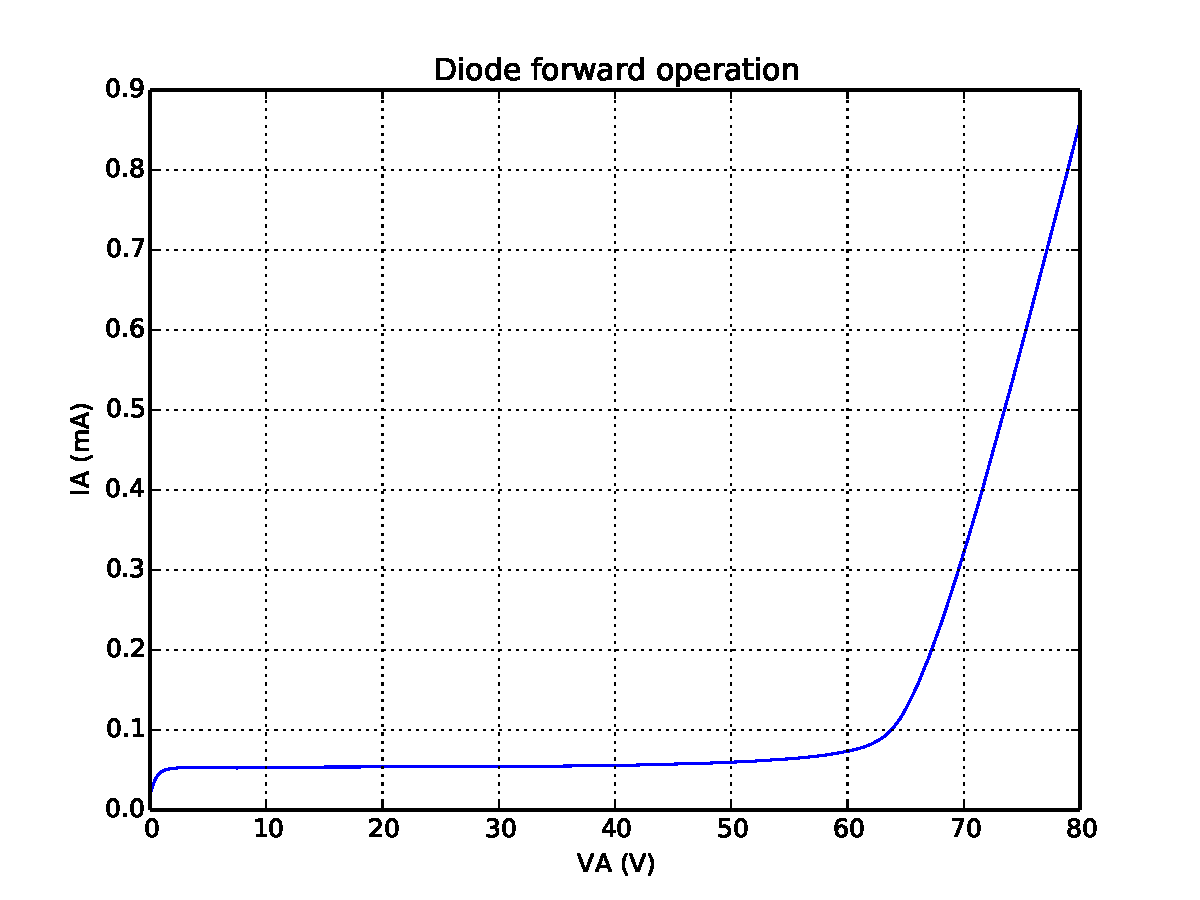
\includegraphics[width=250pt]{Device_plot_data/D7aplot.pdf}};
\node at (15,5) {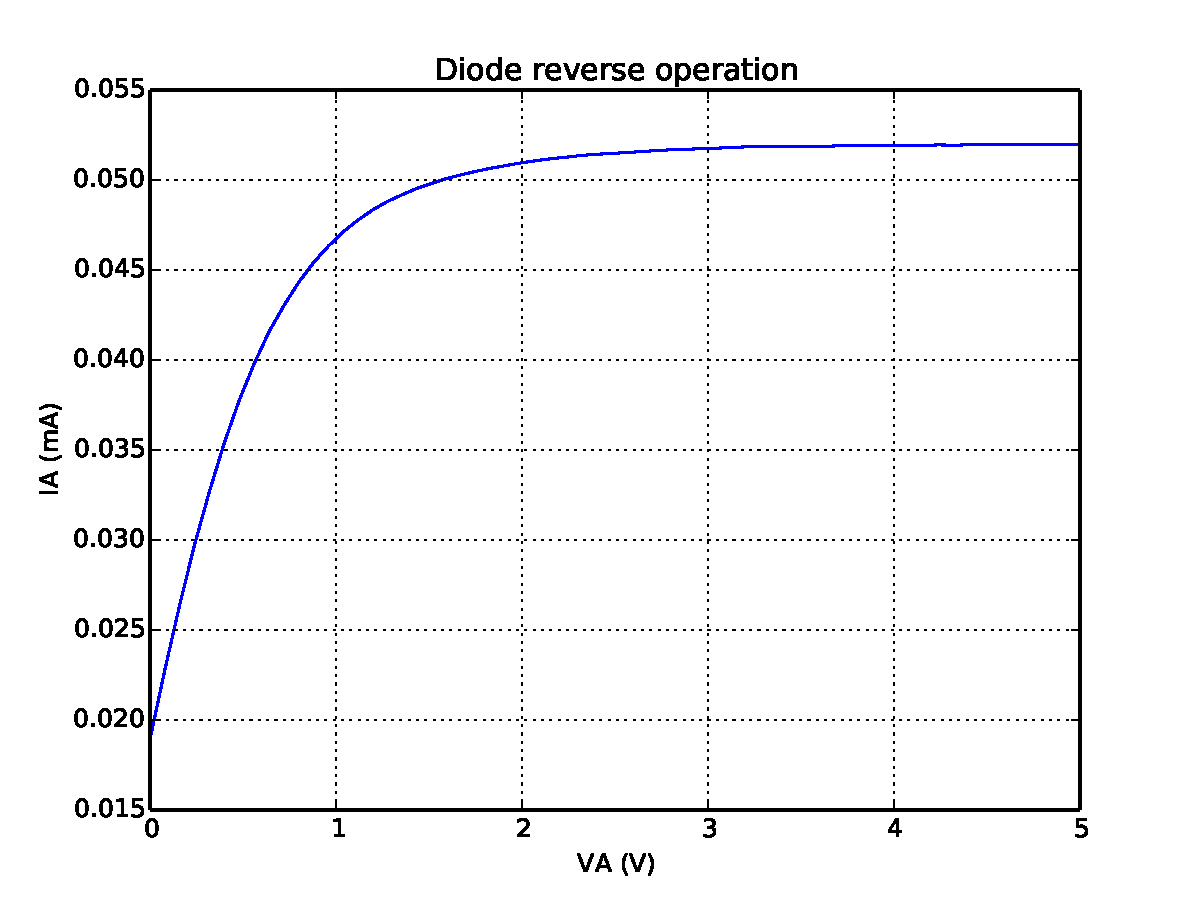
\includegraphics[width=250pt]{Device_plot_data/D7bplot.pdf}};
\end{tikzpicture}
\caption{Plots of forward and reverse operation of Diode 7.}
\end{figure}

Looking at the plots above, the forward turn on voltage is $V_F \approx 70 V$ while the reverse bias turn off voltage is about $V_{RB} \approx 0.5 V$. To calculate the series resistance in the forward bias we look at the region of the curve where V is greater than 65 V. The inverse of the slope there results in $R = 17.8 \,k\Omega$. Similarly for the reverse bias plot, looking at the region below 0.5 Volts, we find that the inverse of the slope is $R = -22.1\,k\Omega$.



\subsection{MOSFETs of Varying Length, [8a-d]} %%%%%%%%%%%%%% MOSFETS 8a-d

\subsubsection{Measurement setups}
\begin{figure}[H]
\centering
\begin{tikzpicture}

\node at (5,5) {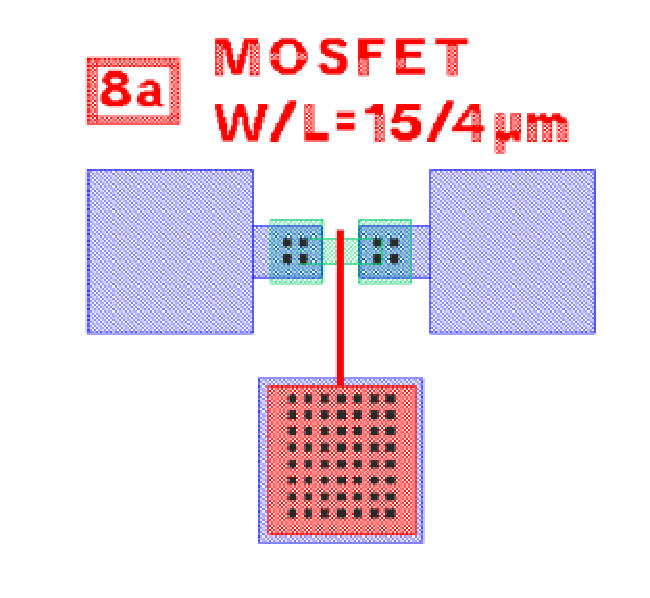
\includegraphics[width=200pt]{Device_setup/device8a2.pdf}};
\node at (15,5) {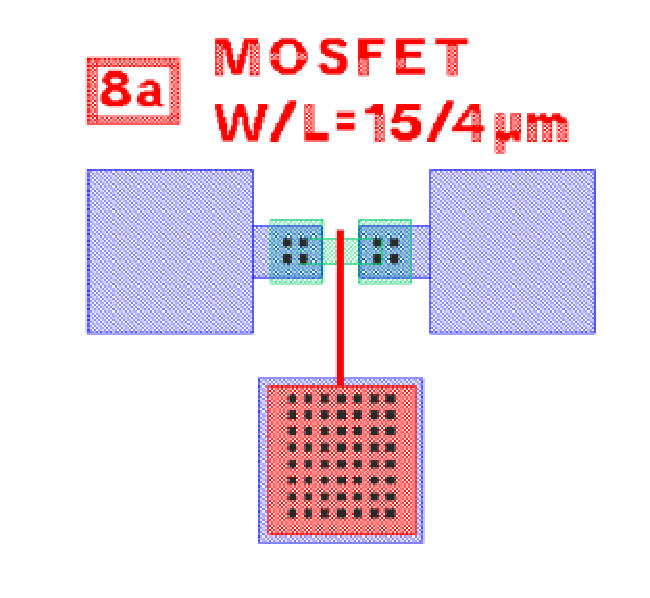
\includegraphics[width=200pt]{Device_setup/device8a2.pdf}};
\node at (5,9) {\textbf{Test 1}};
\node at (15,9) {\textbf{Test 2}};
\node at (3.5,6) {\textbf{D}};
\node at (7,6) {\textbf{S}};
\node at (4.3,3.5) {\textbf{G}};
\draw[<->,thick] (3.4,5) -- (3.4,2.3); % Drain
\node at (3.5,2) {V sweep, 0 to 5 V, measure I, V};
\draw[<->,thick] (7.1,5.5) -- (8,7.3); % source
\node at (8,7.5) {constant};
\draw[<->,thick] (5.5,3) -- (8,3) -- (8,3.3); % Gate
\node at (8.5,3.6) {V sweep, 0 to 5 V, step size 1};
\node at (5,8.5) {Stage connector is GND}; % Stage connector, B
%%%%
\node at (15,8.5) {Stage connector V sweep, 0 to -2 V, step size 2};
\draw[<->,thick] (13.4,5) -- (11.5,6.4); % Drain
\node at (11,6.6) {Constant, comp 0.05, measure I};
\draw[<->,thick] (17.5,5) -- (17.5,3.7);
\node at (17.6,3.5) {Constant};
\draw[<->,thick] (15,3) -- (15,2) -- (11,2) -- (11,2.5);
\node at (11.5,3) {V sweep, 0 to 12 V, measure V};
\end{tikzpicture}
\caption{Measurement setup for Mosfet 8a. The same setup is used for Mosfets 8a-d. The only difference is the channel length which changes from 4 (8a) to 6 (8b) to 8 (8c) to 10 (8d) microns.}
\end{figure}

\subsubsection{Plots of $I_D$-$V_{D}$, sweeping $V_G$}

\begin{figure}[H]
\centering
\begin{tikzpicture}
\node at (-5,5) {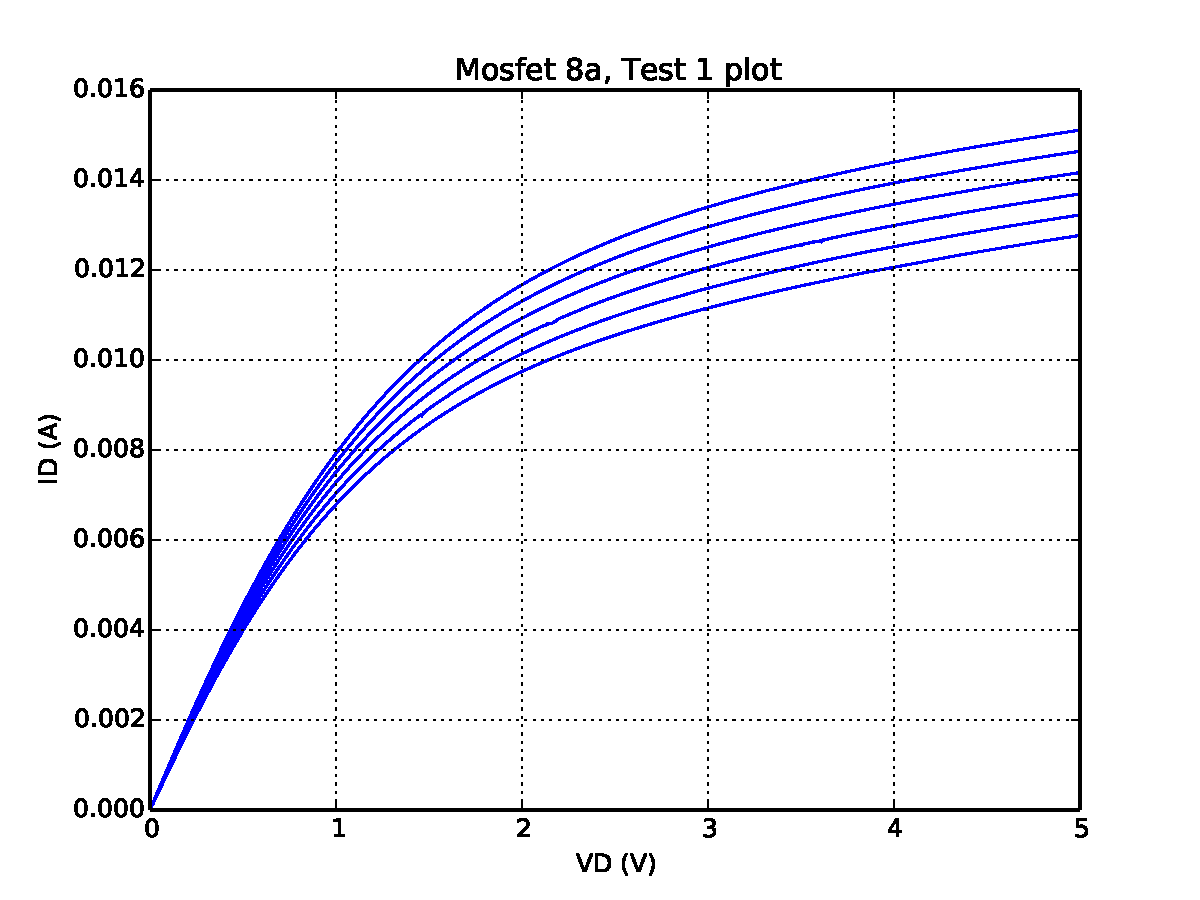
\includegraphics[width=250pt]{Device_plot_data/D8a1plot.pdf}};
\node at (5,5) {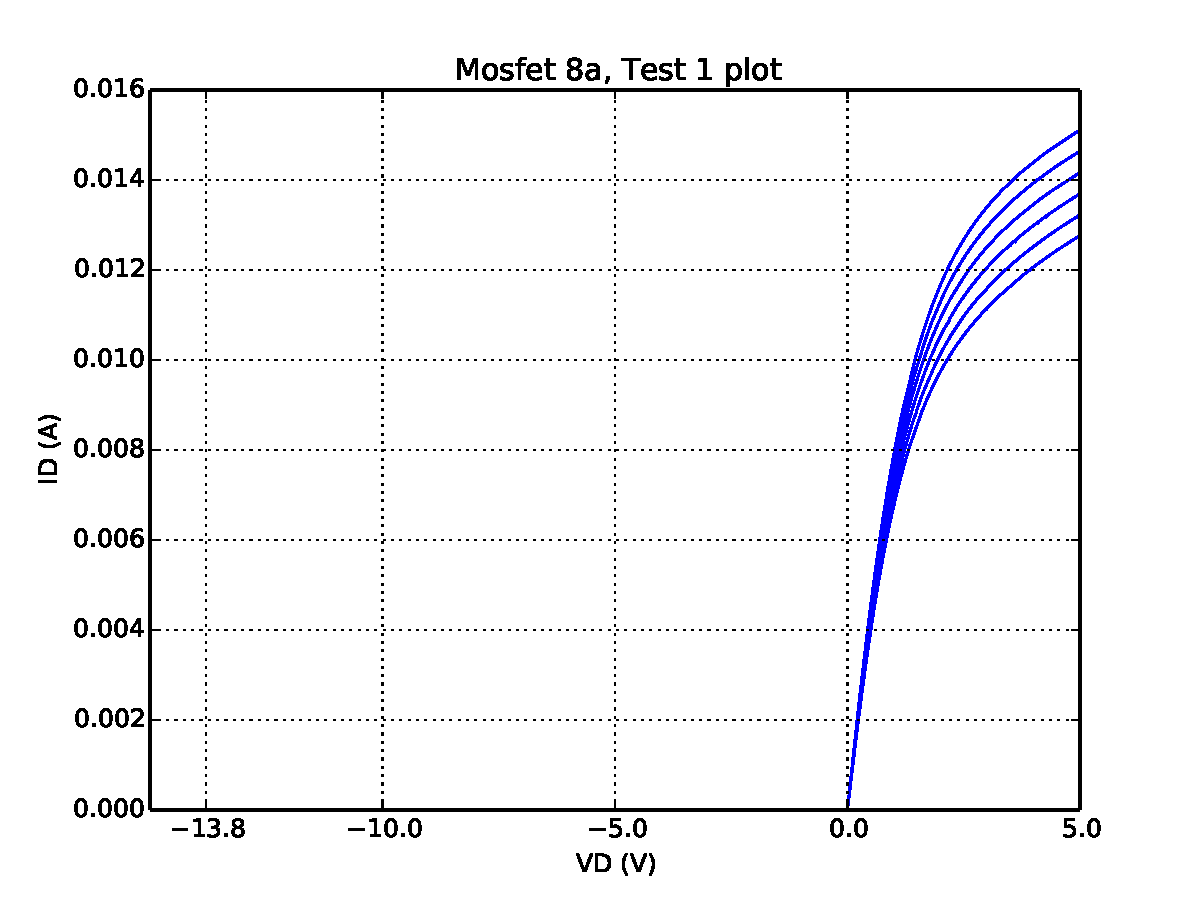
\includegraphics[width=250pt]{Device_plot_data/D8a1longplot.pdf}};
\draw[-,red,dashed] (2.1,2.35) -- (8.5,7.34);
\draw[-,red,dashed] (2.1,2.35) -- (8.5,7.2);
\draw[-,red,dashed] (2.1,2.35) -- (8.5,7.025);
\draw[-,red,dashed] (2.1,2.35) -- (8.5,6.88);
\draw[-,red,dashed] (2.1,2.35) -- (8.5,6.72);
\draw[-,red,dashed] (2.1,2.35) -- (8.5,6.57);
\end{tikzpicture}
\caption{Test 1 for Mosfet 8a with extended x axis range in order to calculate lambda.}
\label{fig:8along}
\end{figure} 
We see that everything intersects at about -13.8 V. This corresponds to $\lambda = \frac{1}{-13.8} = -0.0725$.

\begin{figure}[H]
\centering
\begin{tikzpicture}
\node at (-5,5) {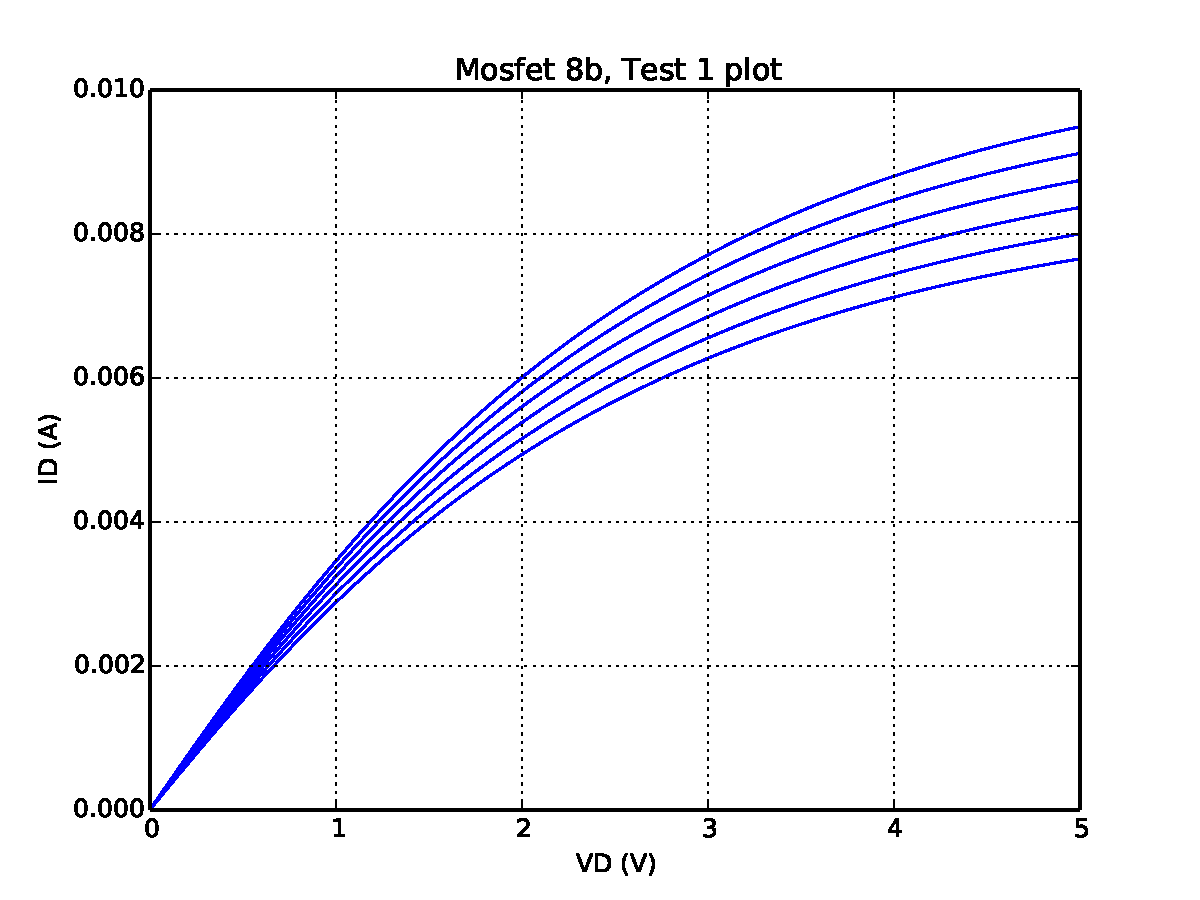
\includegraphics[width=250pt]{Device_plot_data/D8b1plot.pdf}};
\node at (5,5) {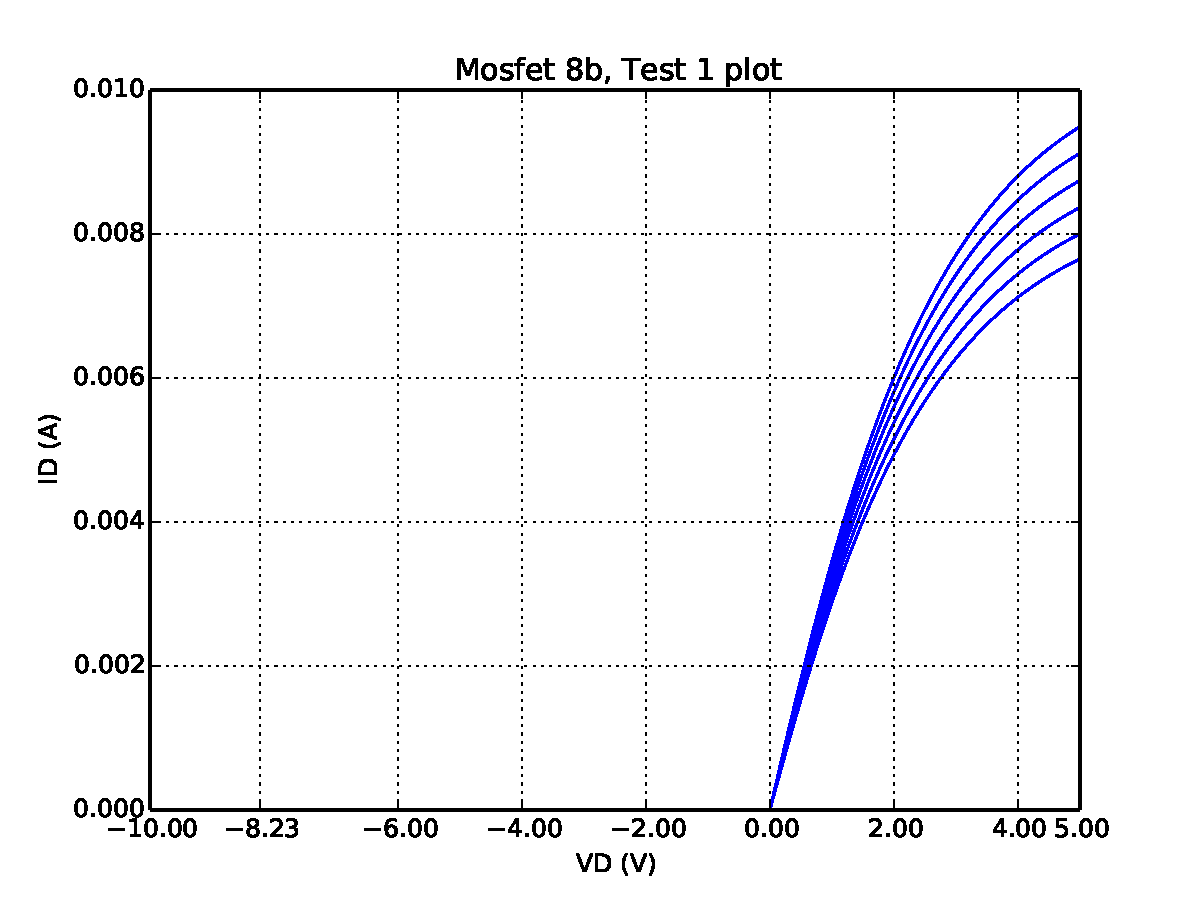
\includegraphics[width=250pt]{Device_plot_data/D8b1longplot.pdf}};
\draw[-,red,dashed] (2.5,2.35) -- (8.5,7.37);
\draw[-,red,dashed] (2.5,2.35) -- (8.5,7.18);
\draw[-,red,dashed] (2.5,2.35) -- (8.5,6.99);
\draw[-,red,dashed] (2.5,2.35) -- (8.5,6.78);
\draw[-,red,dashed] (2.5,2.35) -- (8.5,6.60);
\draw[-,red,dashed] (2.5,2.35) -- (8.5,6.41);
\end{tikzpicture}
\caption{Test 1 for Mosfet 8b with extended x axis range in order to calculate lambda.}
\label{fig:8blong}
\end{figure}
We see that everything intersects at about -8.23 V. This corresponds to $\lambda = \frac{1}{-8.23} = -0.122$.


\begin{figure}[H]
\centering
\begin{tikzpicture}
\node at (-5,5) {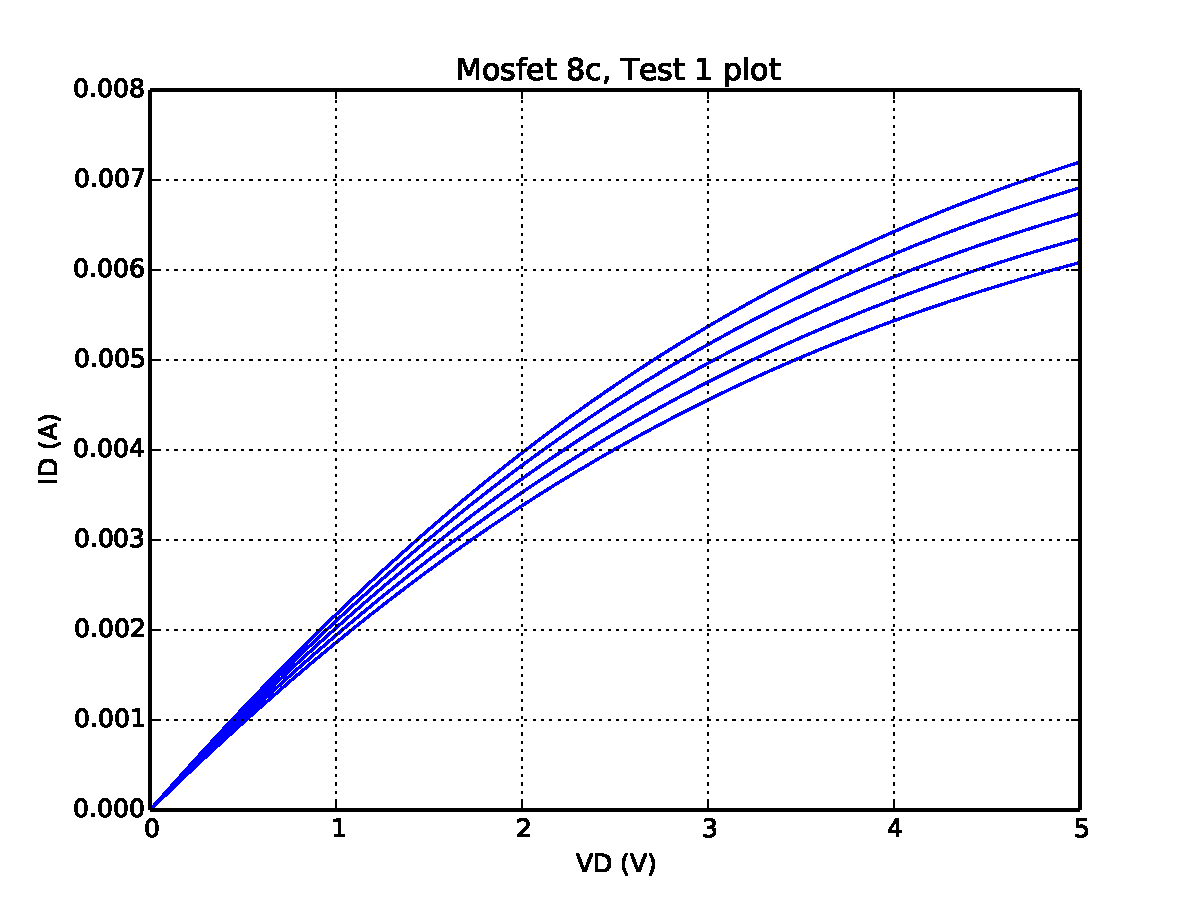
\includegraphics[width=250pt]{Device_plot_data/D8c1plot.pdf}};
\node at (5,5) {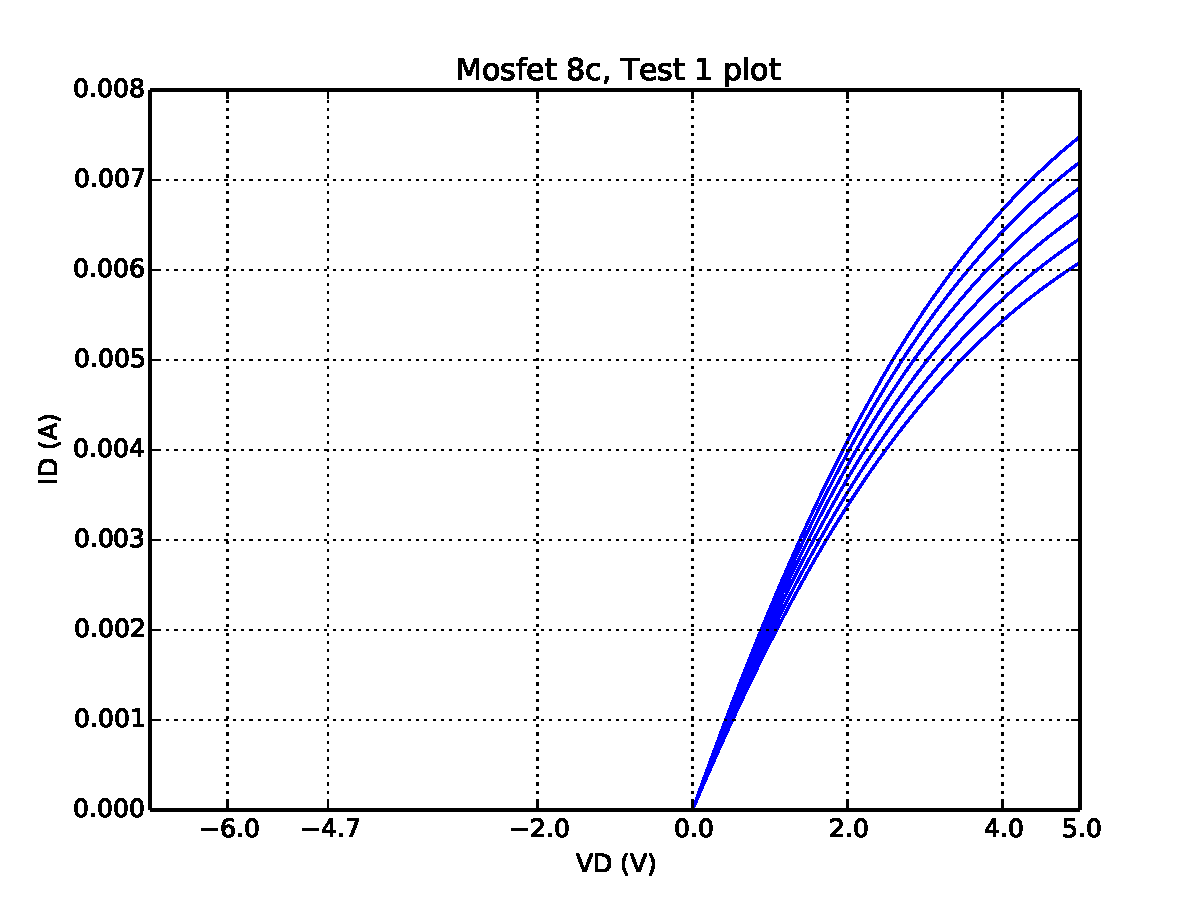
\includegraphics[width=250pt]{Device_plot_data/D8c1longplot.pdf}};
\draw[-,red,dashed] (3,2.35) -- (8.5,7.3);
\draw[-,red,dashed] (3,2.35) -- (8.5,7.1);
\draw[-,red,dashed] (3,2.35) -- (8.5,6.92);
\draw[-,red,dashed] (3,2.35) -- (8.5,6.73);
\draw[-,red,dashed] (3,2.35) -- (8.5,6.55);
\draw[-,red,dashed] (3,2.35) -- (8.5,6.37);
\end{tikzpicture}
\caption{Test 1 for Mosfet 8c with extended x axis range in order to calculate lambda.}
\label{fig:8clong}
\end{figure}
We see that everything intersects at about -4.70 V. This corresponds to $\lambda = \frac{1}{-4.70} = -0.213$.


\begin{figure}[H]
\centering
\begin{tikzpicture}
\node at (-5,5) {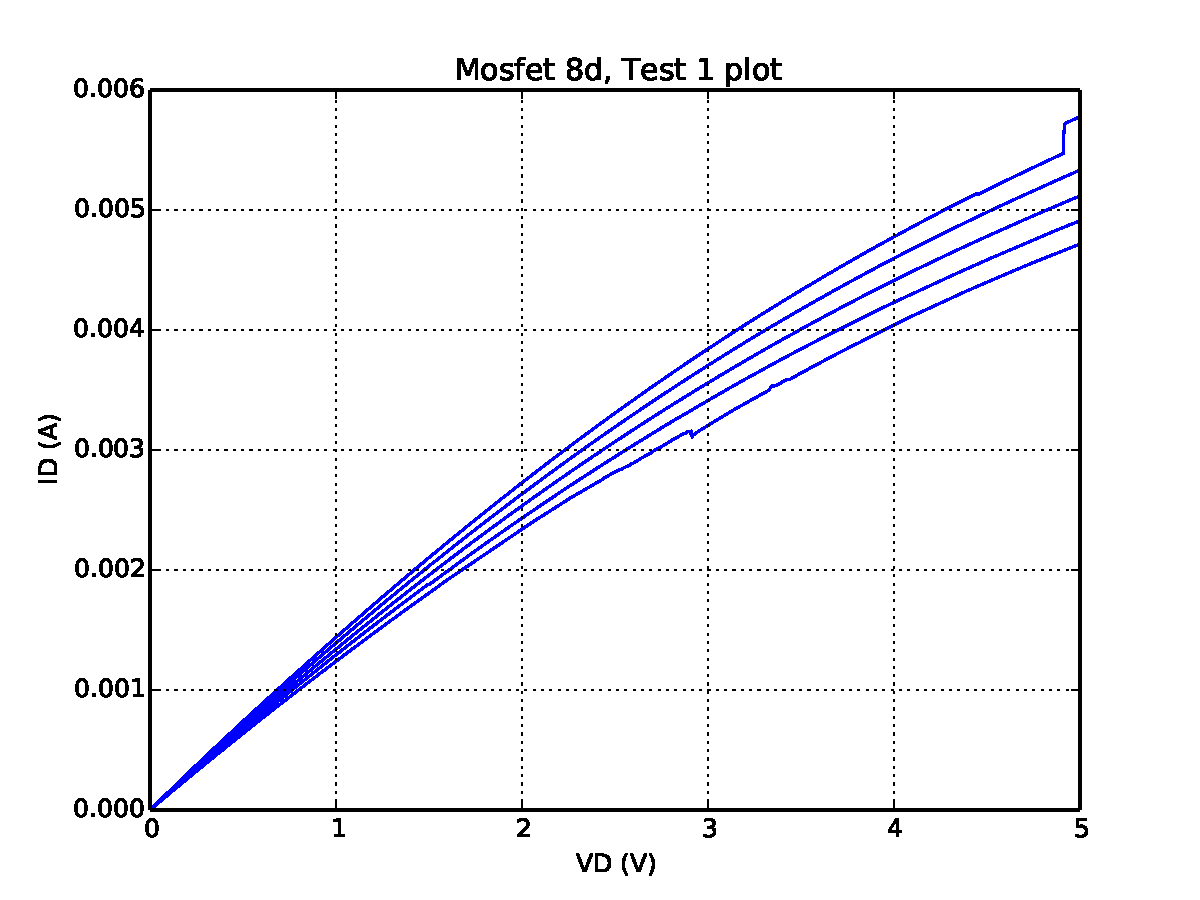
\includegraphics[width=250pt]{Device_plot_data/D8d1plot.pdf}};
\node at (5,5) {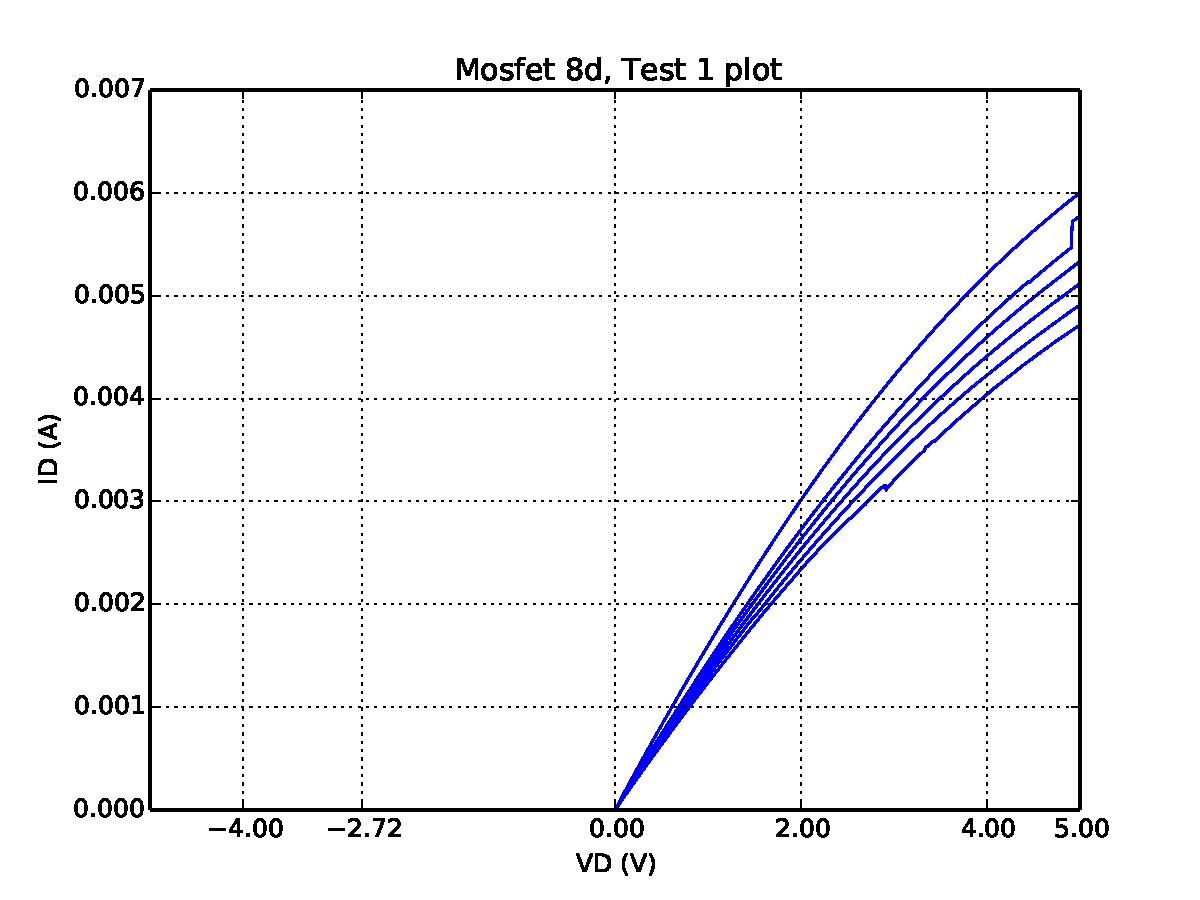
\includegraphics[width=250pt]{Device_plot_data/D8d1longplot.pdf}};
\draw[-,red,dashed] (3.25,2.35) -- (8.5,6.87);
\draw[-,red,dashed] (3.25,2.35) -- (8.5,6.525);
\draw[-,red,dashed] (3.25,2.35) -- (8.5,6.365);
\draw[-,red,dashed] (3.25,2.35) -- (8.5,6.21);
\draw[-,red,dashed] (3.25,2.35) -- (8.5,6.05);
\draw[-,red,dashed] (3.25,2.35) -- (8.5,5.90);
\end{tikzpicture}
\caption{Test 1 for Mosfet 8d with extended x axis range in order to calculate lambda.}
\label{fig:8dlong}
\end{figure}
We see that everything intersects at about -2.72 V. This corresponds to $\lambda = \frac{1}{-2.72} = -0.368$.

\subsubsection{$\lambda$ vs $L_{\text{Drawn}}$}
To summarize, here is a table of all $\lambda$ values calculated,
\begin{figure}[H]
\centering
\begin{tabular}{c || c | c | c }
MOSFET device & $\lambda$ ($V^{-1}$) & $L_{\text{drawn}}$ ($\mu m$) & Fig \# \\ \hline
8a & -0.0725 & 4 & \textcolor{blue}{\ref{fig:8along}} \\ \hline
8b & -0.122 & 6 & \textcolor{blue}{\ref{fig:8blong}}\\ \hline
8c & -0.213 & 8 & \textcolor{blue}{\ref{fig:8clong}}\\ \hline
8d & -0.368 & 10 & \textcolor{blue}{\ref{fig:8dlong}}\\ \hline
\end{tabular}
\caption{all $\lambda$ values for mosfets 9a-d along with gate lengths.}
\end{figure}

\begin{figure}[H]
\centering
\begin{tikzpicture}
\node at (5,5) {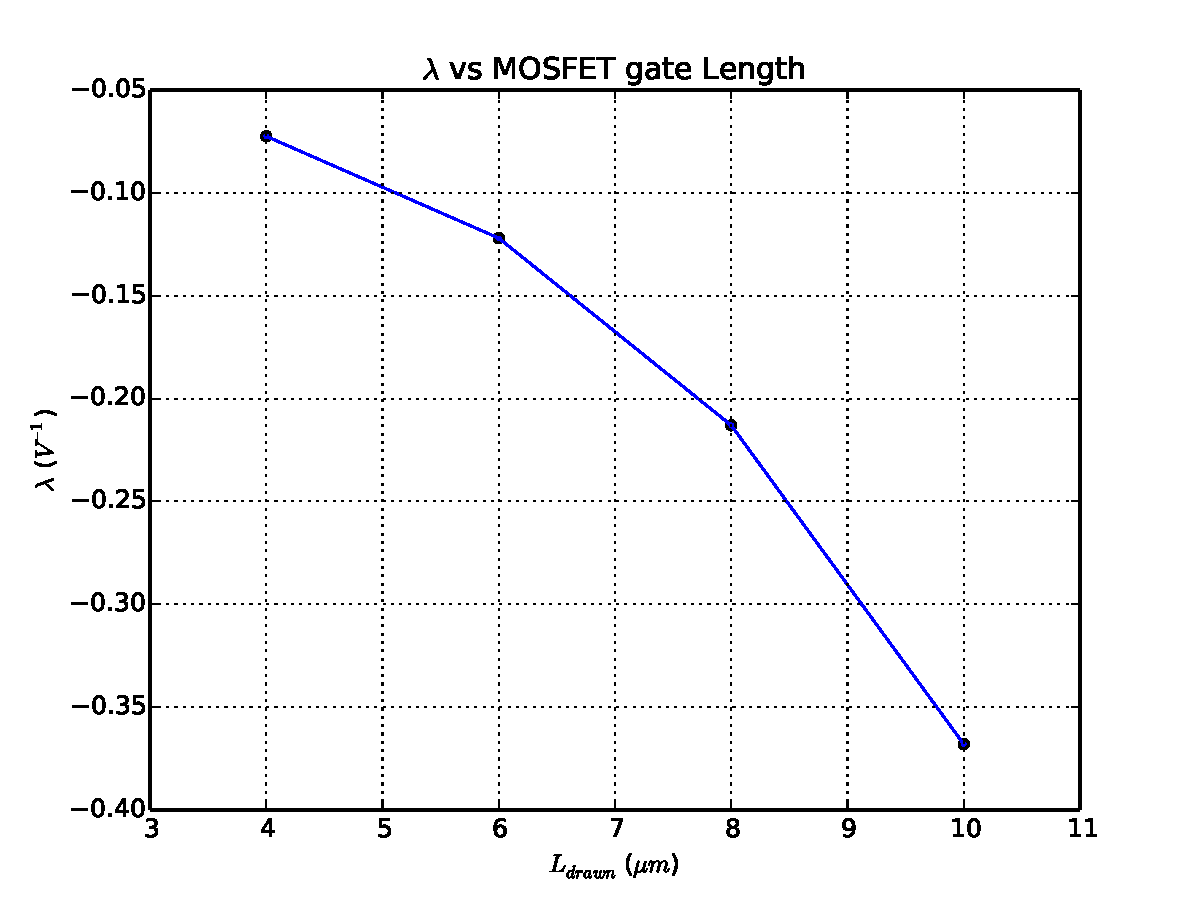
\includegraphics[width=250pt]{Device_plot_data/D8plot.pdf}};
\end{tikzpicture}
\caption{$\lambda$ for each 8a-d device vs the gate length.}
\end{figure}


\subsubsection{Plots of $I_D$-$V_G$, sweeping $V_B$}

\begin{figure}[H]
\centering
\begin{tikzpicture}
\node at (5,5) {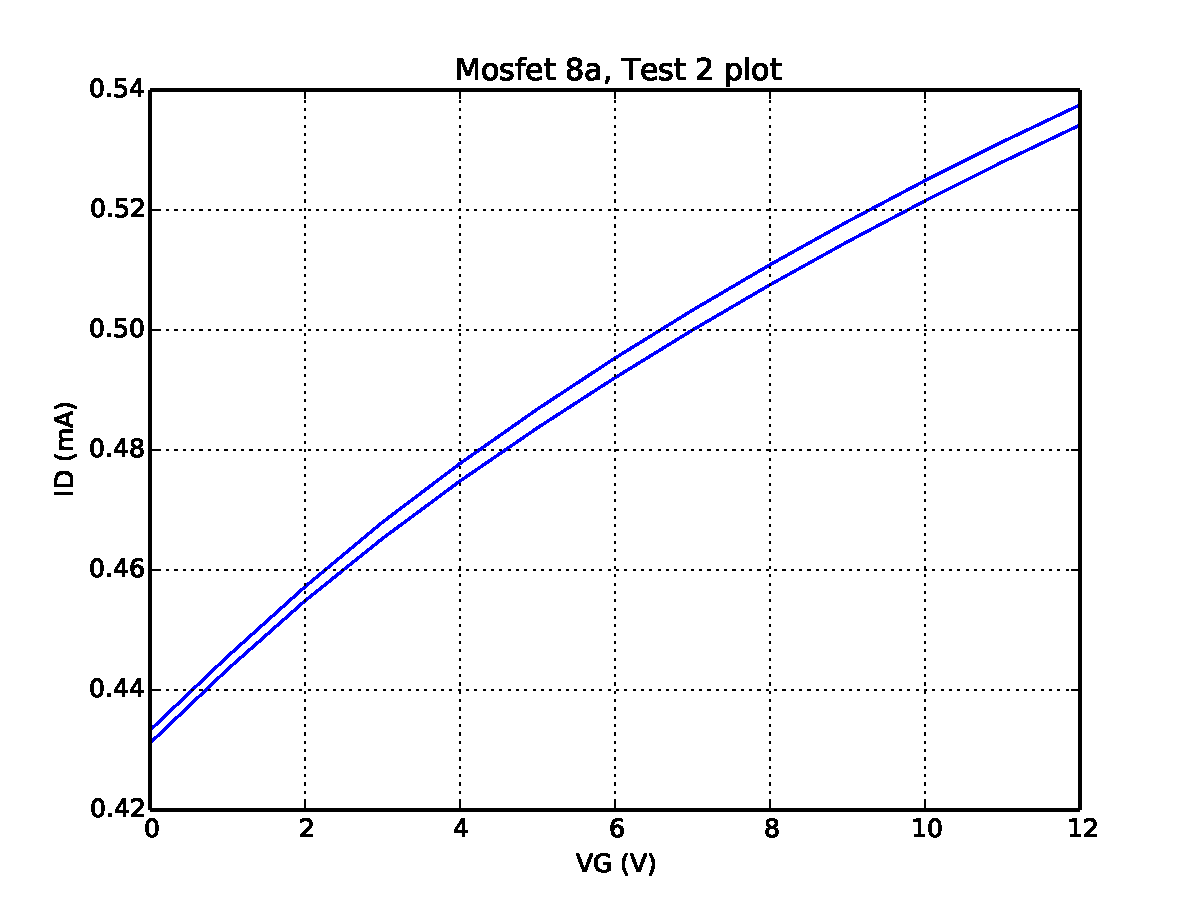
\includegraphics[width=250pt]{Device_plot_data/D8a2plot.pdf}};
\node at (15,5) {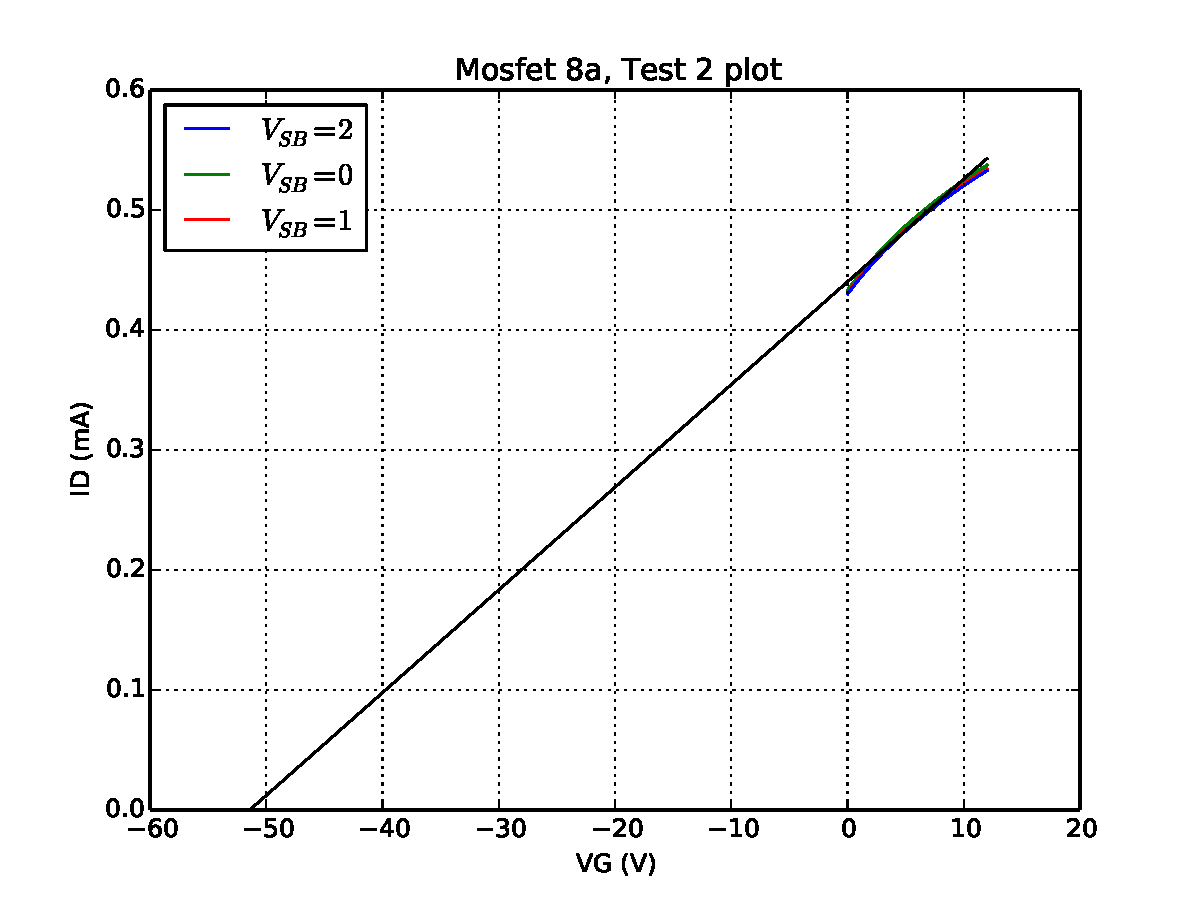
\includegraphics[width=250pt]{Device_plot_data/D8a2linplot.pdf}};
\end{tikzpicture}
\caption{Test 2 for Mosfet 8a. On the right side we did a linear regression on the $V_{SB} = 0$ line in order to get a estimate of the threshold voltage.}
\label{fig:8alin}
\end{figure}

Since it is quite difficult to see where a slope change occurs in order to find the threshold voltage, we can do a linear regression using the $V_{SB} = 0$ line. With linear regression, $V_t = -51.4 V$. One reason why there is no slope change might have to do with the fact that most of our MOSFETS show characteristics of junction leakage.

\begin{figure}[H]
\centering
\begin{tikzpicture}
\node at (5,5) {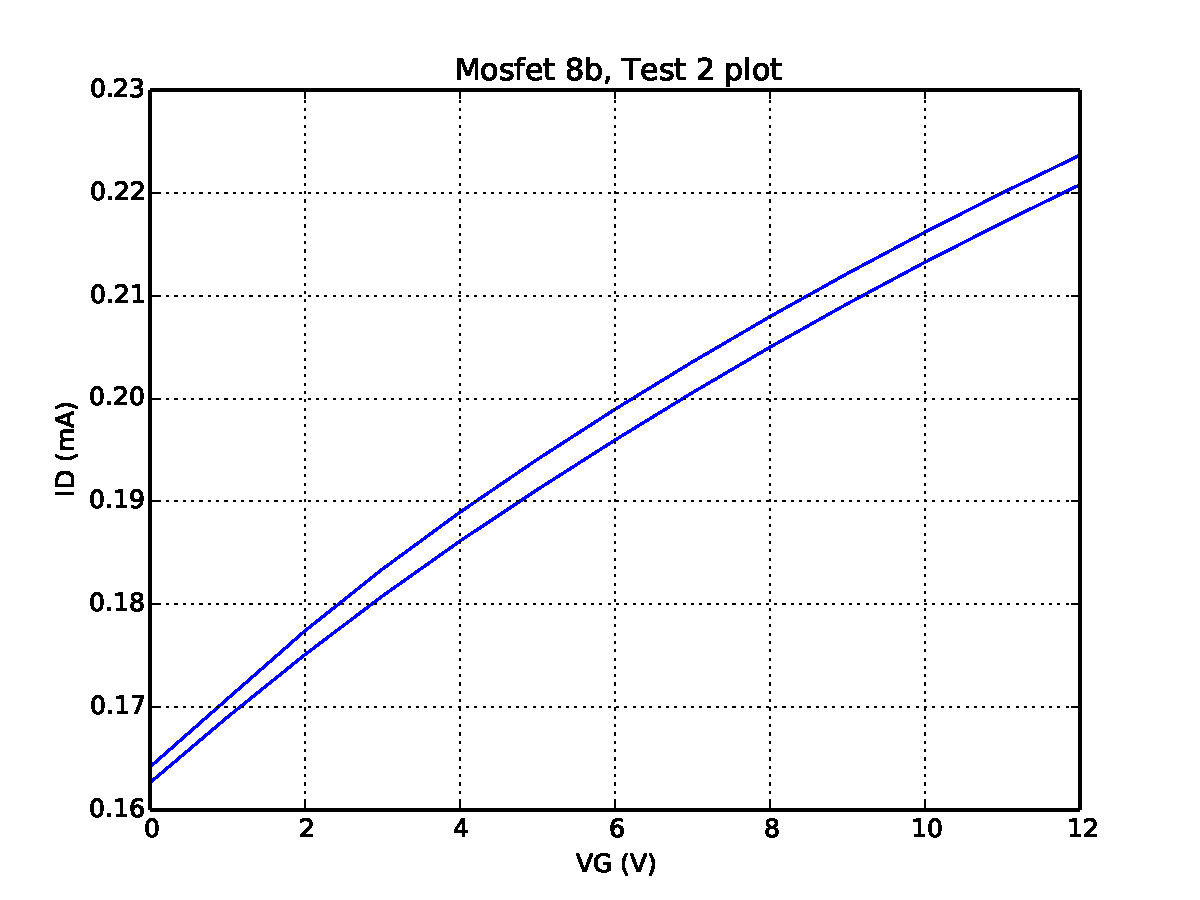
\includegraphics[width=250pt]{Device_plot_data/D8b2plot.pdf}};
\node at (15,5) {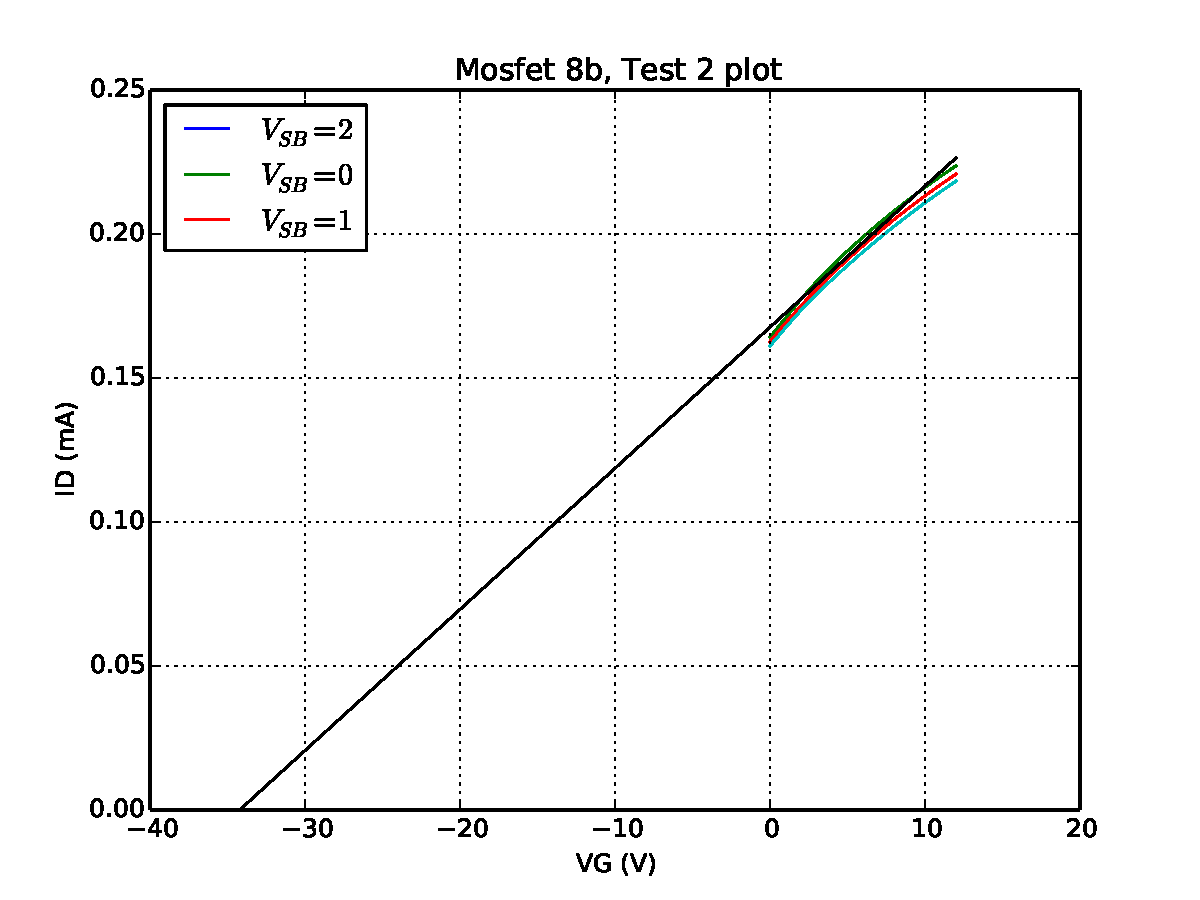
\includegraphics[width=250pt]{Device_plot_data/D8b2linplot.pdf}};
\end{tikzpicture}
\caption{Test 2 for Mosfet 8b. On the right side we did a linear regression on the $V_{SB} = 0$ line in order to get a estimate of the threshold voltage.}
\label{fig:8blin}
\end{figure}

Similarly, the threshold voltage is not clear in the figure above. Using linear regression again with $V_{SB} = 0$ we get $V_t = -34.2$.

\begin{figure}[H]
\centering
\begin{tikzpicture}
\node at (5,5) {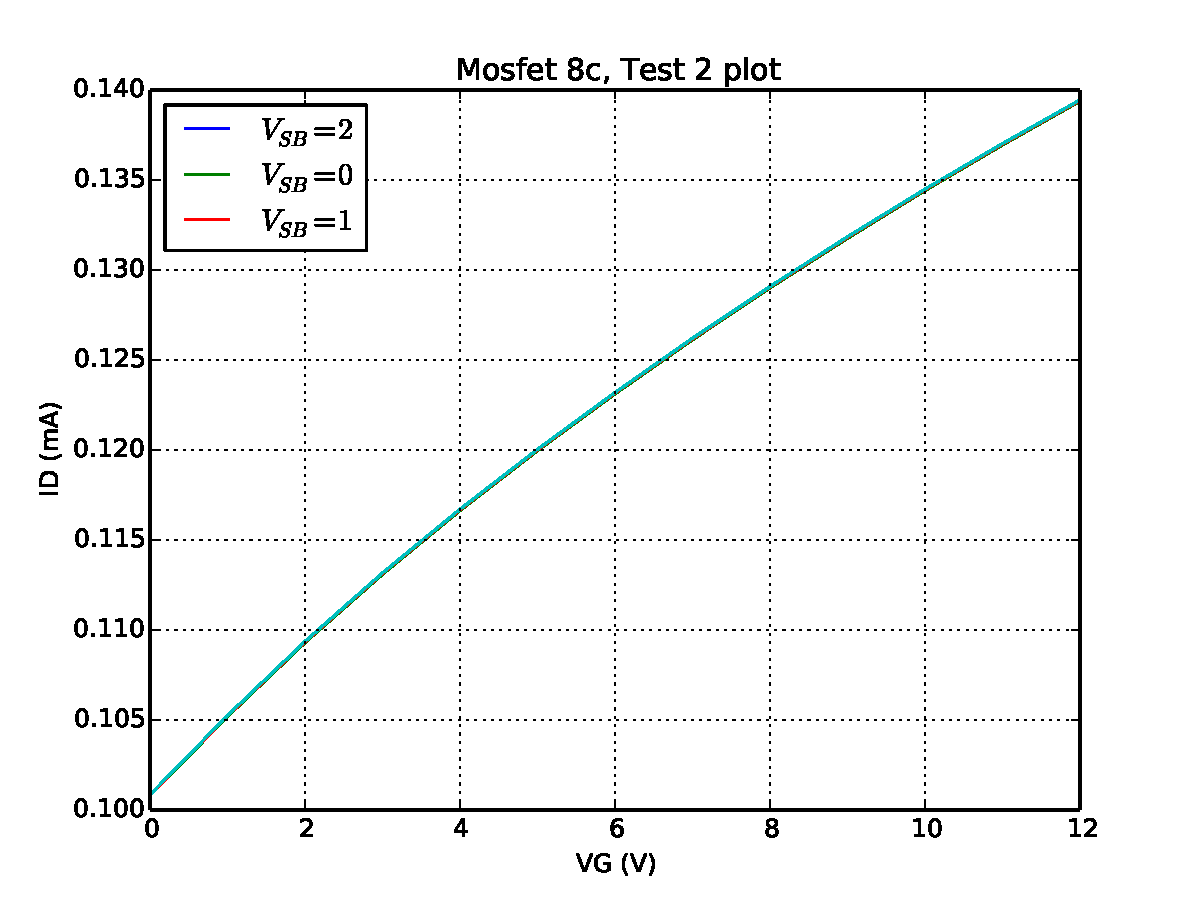
\includegraphics[width=250pt]{Device_plot_data/D8c2plot.pdf}};
\node at (15,5) {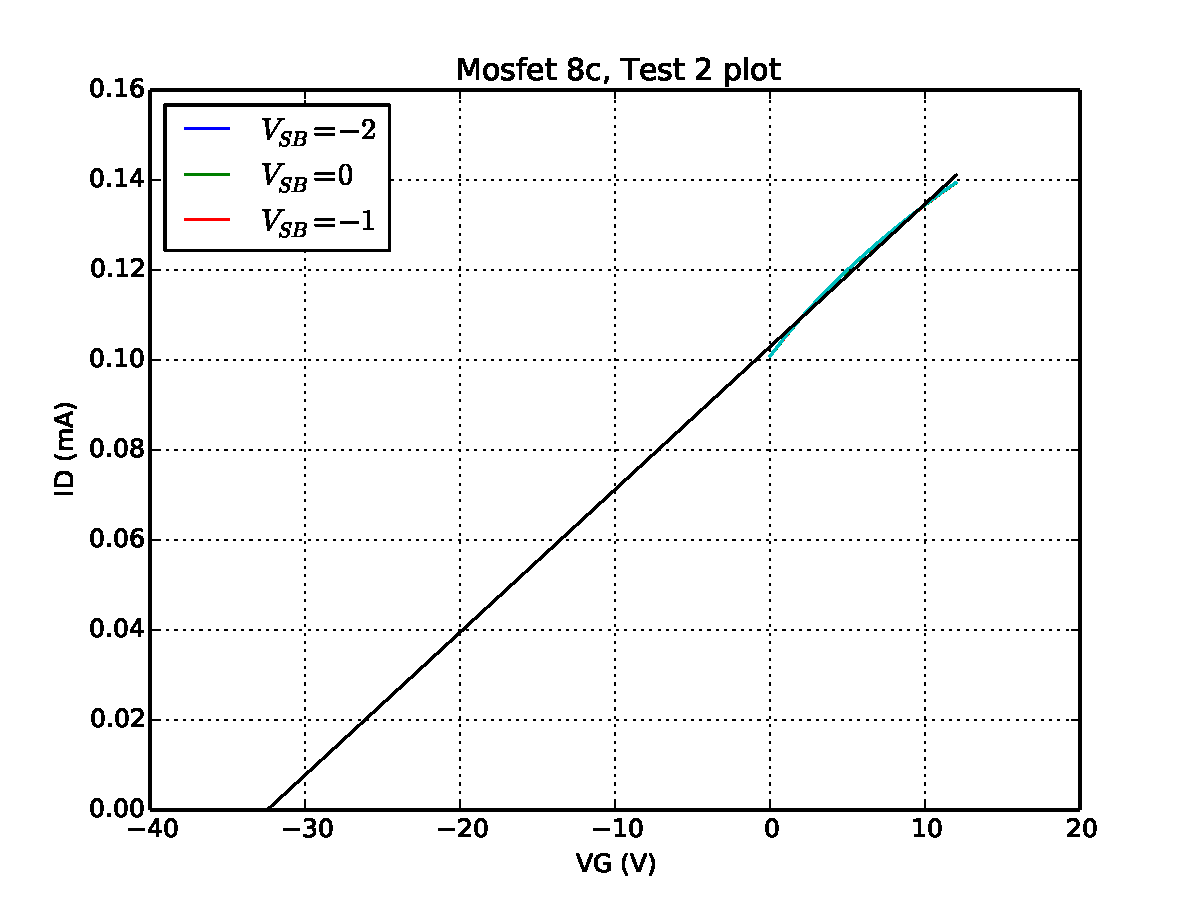
\includegraphics[width=250pt]{Device_plot_data/D8c2linplot.pdf}};
\end{tikzpicture}
\caption{Test 2 for Mosfet 8c. On the right side we did a linear regression on the $V_{SB} = 0$ line in order to get a estimate of the threshold voltage.}
\label{fig:8clin}
\end{figure}

Similarly, the threshold voltage is not clear in the figure above. Using linear regression again with $V_{SB} = 0$ we get $V_t = -32.4$.

\begin{figure}[H]
\centering
\begin{tikzpicture}
\node at (5,5) {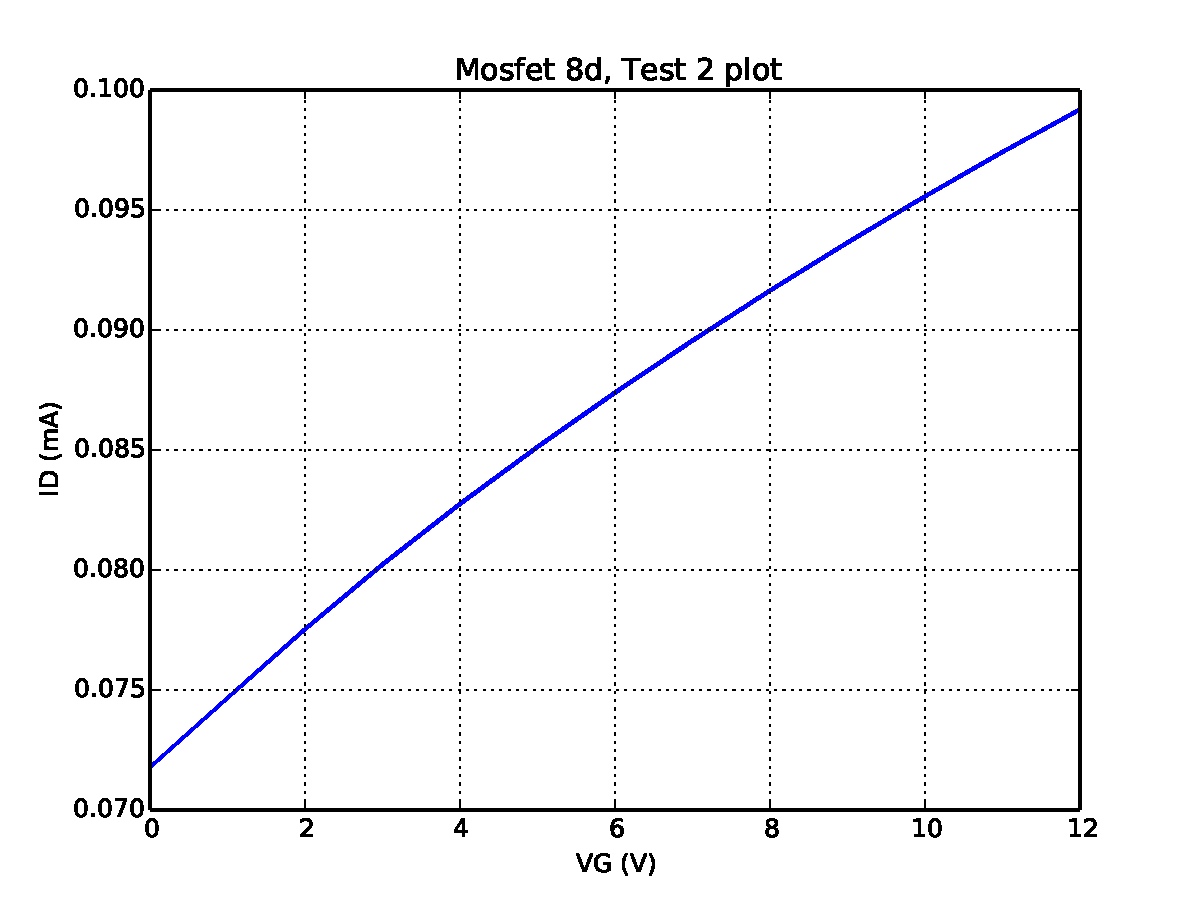
\includegraphics[width=250pt]{Device_plot_data/D8d2plot.pdf}};
\node at (15,5) {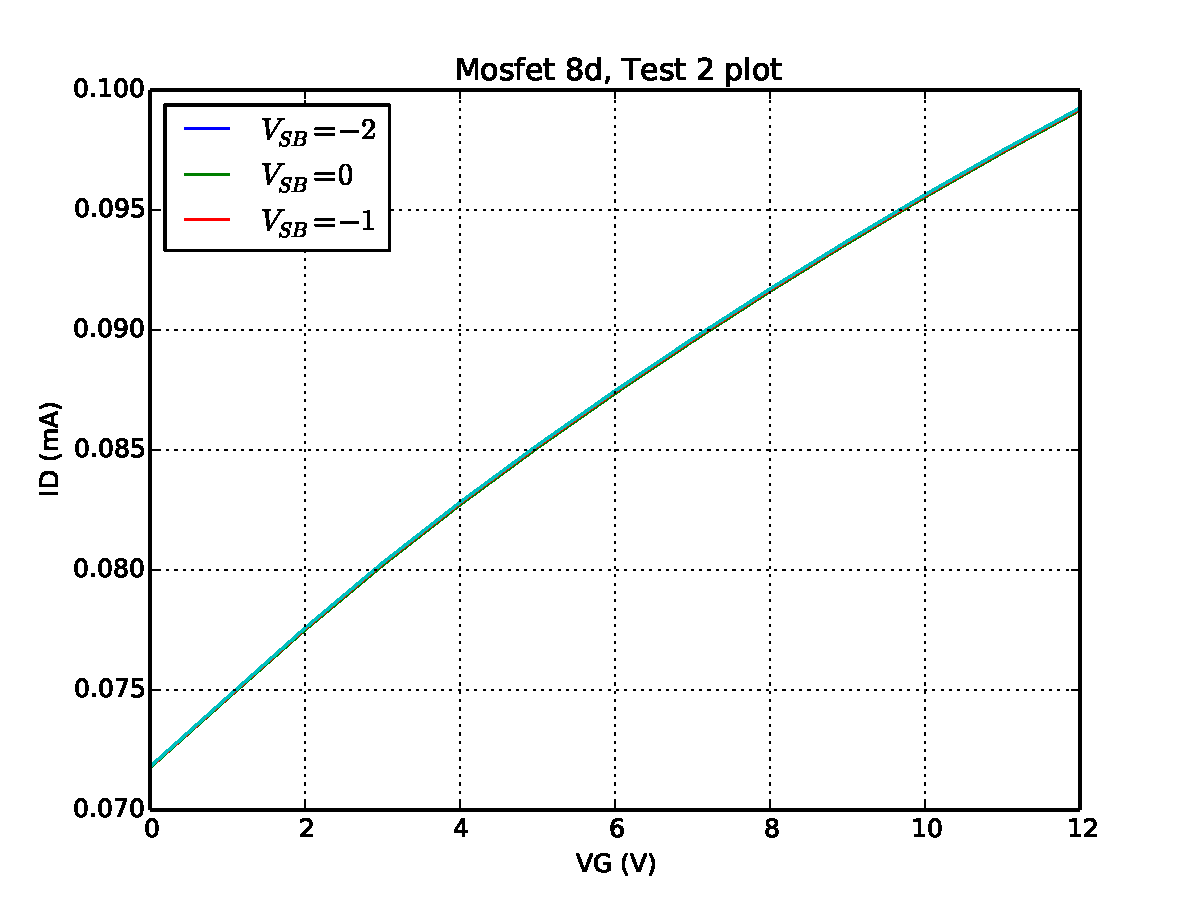
\includegraphics[width=250pt]{Device_plot_data/D8d2linplot.pdf}};
\end{tikzpicture}
\caption{Test 2 for Mosfet 8d. On the right side we did a linear regression on the $V_{SB} = 0$ line in order to get a estimate of the threshold voltage.}
\label{fig:8dlin}
\end{figure}

Similarly, the threshold voltage is not clear in the figure above. Using linear regression again with $V_{SB} = 0$ we get $V_t = -32.2$.

\subsubsection{Estimate of $\Delta L$}
To summarize the threshold voltages calculated in the last section,
\begin{figure}[H]
\centering
\begin{tabular}{c || c | c | c }
MOSFET device & $V_t (V)$ & $L_{\text{drawn}}$ ($\mu m$) & Fig \# \\ \hline
8a & -51.4 & 4 & \textcolor{blue}{\ref{fig:8alin}} \\ \hline
8b & -34.2 & 6 & \textcolor{blue}{\ref{fig:8blin}}\\ \hline
8c & -32.4 & 8 & \textcolor{blue}{\ref{fig:8clin}}\\ \hline
8d & -32.2 & 10 & \textcolor{blue}{\ref{fig:8dlin}}\\ \hline
\end{tabular}
\caption{Threshold voltages for all MOSFET 8 devices.}
\end{figure}

Now the first step in calculating $\Delta L$ is to find the extended Resistance. We can do this by plotting the measured resistance vs gate Length at various voltages (from lecture). This plot looks like the following:
\begin{figure}[H]
\centering
\begin{tikzpicture}
\node at (5,5) {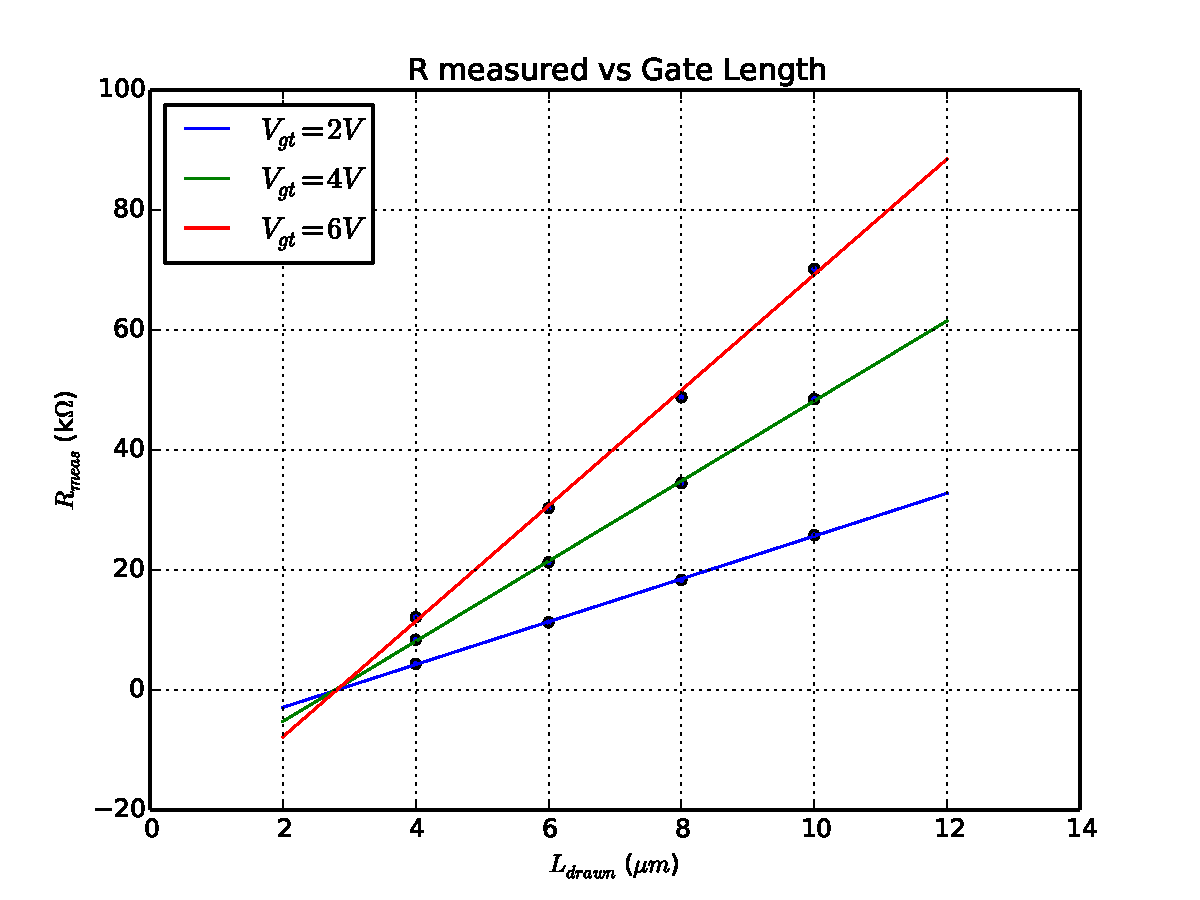
\includegraphics[width=250pt]{Device_plot_data/D8Rplot.pdf}};
\end{tikzpicture}
\caption{Measured Resistance vs Gate length for various lengths and voltages}
\end{figure}
The Y value from the origin (0) to the point of intersection would be the extended Resistance value. However in our case the lines intersect at just about 0; this means that $R_{\text{ext}} \approx 0$. Now we can solve for $\Delta L$ by using the following equation from lecture:
\begin{equation}
R_{\text{meas}} = \frac{L_{\text{drawn}} - \Delta L}{\mu W C_{\text{gox}} (V_{\text{gs}} - V_t)} + R_{\text{ext}}
\end{equation}
Solving for $\Delta L$ and noting that from earlier that $C_{\text{gox}} = 1.95$pF/${\mu m}^{2}$ and $\mu_n = 92.4 {\text{cm}}^{2}$/V-s. We will also choose $V_{gs} - V_t = 2 V$, $L_{\text{drawn}} = 4 \mu m$, and $R_{\text{meas}} = 8.368 k\Omega$. Note that W = 15 $\mu m$ and $R_{ext} = 0$.
\begin{align*}
\Delta L = L_{\text{drawn}} - R_{\text{meas}}\mu_n C_{\text{gox}} (V_{\text{gs}} - V_t) = (8.368\e{3}\Omega)(92.4 {\text{cm}}^{2}/\text{V-s})(15\e{-6}\text{m})(1.95\e{-7}\text{F}/{\text{cm}}^{2})(2\text{V}) = 1.59 \,\mu m
\end{align*}

\subsection{MOSFETs of varying width [9a-c]} %%%%%%%%%%%%%% MOSFETS 9a-c

\subsubsection{Measurement setup}
\begin{figure}[H]
\centering
\begin{tikzpicture}

\node at (5,5) {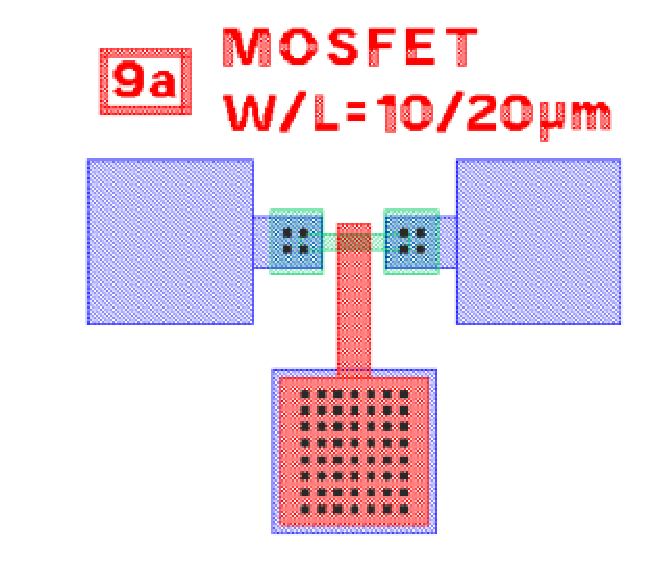
\includegraphics[width=200pt]{Device_setup/device9a2.pdf}};
\node at (15,5) {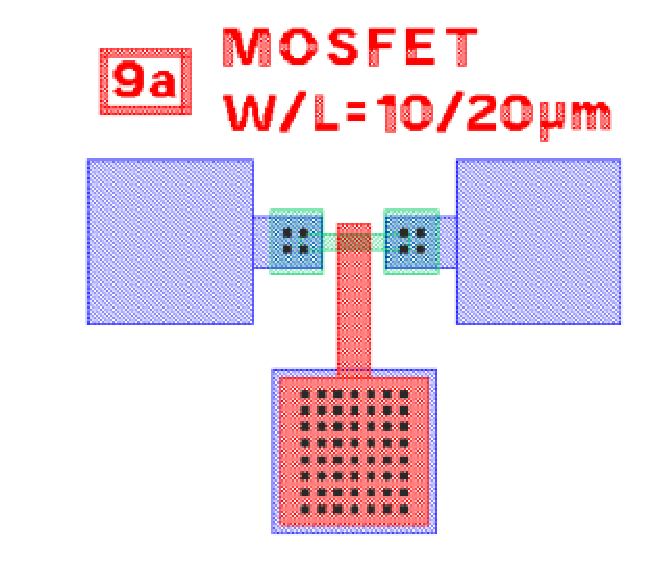
\includegraphics[width=200pt]{Device_setup/device9a2.pdf}};
\node at (5,9) {\textbf{Test 1}};
\node at (15,9) {\textbf{Test 2}};
\node at (3.5,6) {\textbf{D}};
\node at (7,6) {\textbf{S}};
\node at (4.3,3.5) {\textbf{G}};
\draw[<->,thick] (3.4,5) -- (3.4,2.3); % Drain
\node at (3.5,2) {V sweep, 0 to 5 V, measure I, V};
\draw[<->,thick] (7.1,5.5) -- (8,7.3); % source
\node at (8,7.5) {constant};
\draw[<->,thick] (5.5,3) -- (8,3) -- (8,3.3); % Gate
\node at (8.5,3.6) {V sweep, 0 to 5 V, step size 1};
\node at (5,8.5) {Stage connector is GND}; % Stage connector, B
%%%%
\node at (15,8.5) {Stage connector V sweep, 0 to -2 V, step size 2};
\draw[<->,thick] (13.4,5) -- (11.5,6.4); % Drain
\node at (11,6.6) {Constant, comp 0.05, measure I};
\draw[<->,thick] (17.5,5) -- (17.5,3.7);
\node at (17.6,3.5) {Constant};
\draw[<->,thick] (15,3) -- (15,2) -- (11,2) -- (11,2.5);
\node at (11.5,3) {V sweep, 0 to 12 V, measure V};
\end{tikzpicture}
\caption{Measurement setup for Mosfet 9a. The same setup is used for Mosfets 9a-c. The only difference is the channel widths which changes from 10 (9a) to 15 (9b) to 20 (9c) microns.}
\end{figure}

\subsubsection{Plots of $I_D$-$V_D$, sweeping $V_G$ }
\begin{figure}[H]
\centering
\begin{tikzpicture}
\node at (5,5) {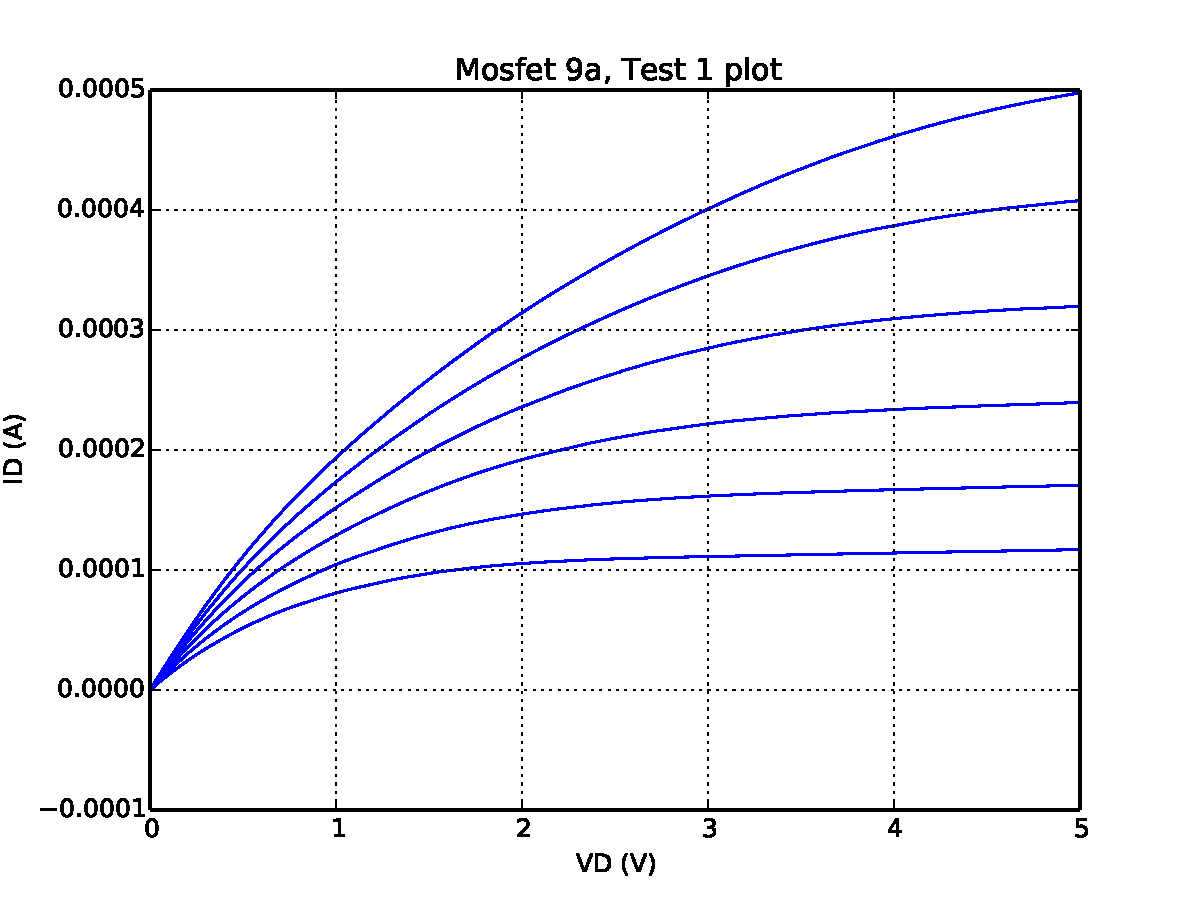
\includegraphics[width=250pt]{Device_plot_data/D9a1plot.pdf}};
\end{tikzpicture}
\caption{Test 1 for Mosfet 9a}
\end{figure}

Calculate stuff here... 

\begin{figure}[H]
\centering
\begin{tikzpicture}
\node at (5,5) {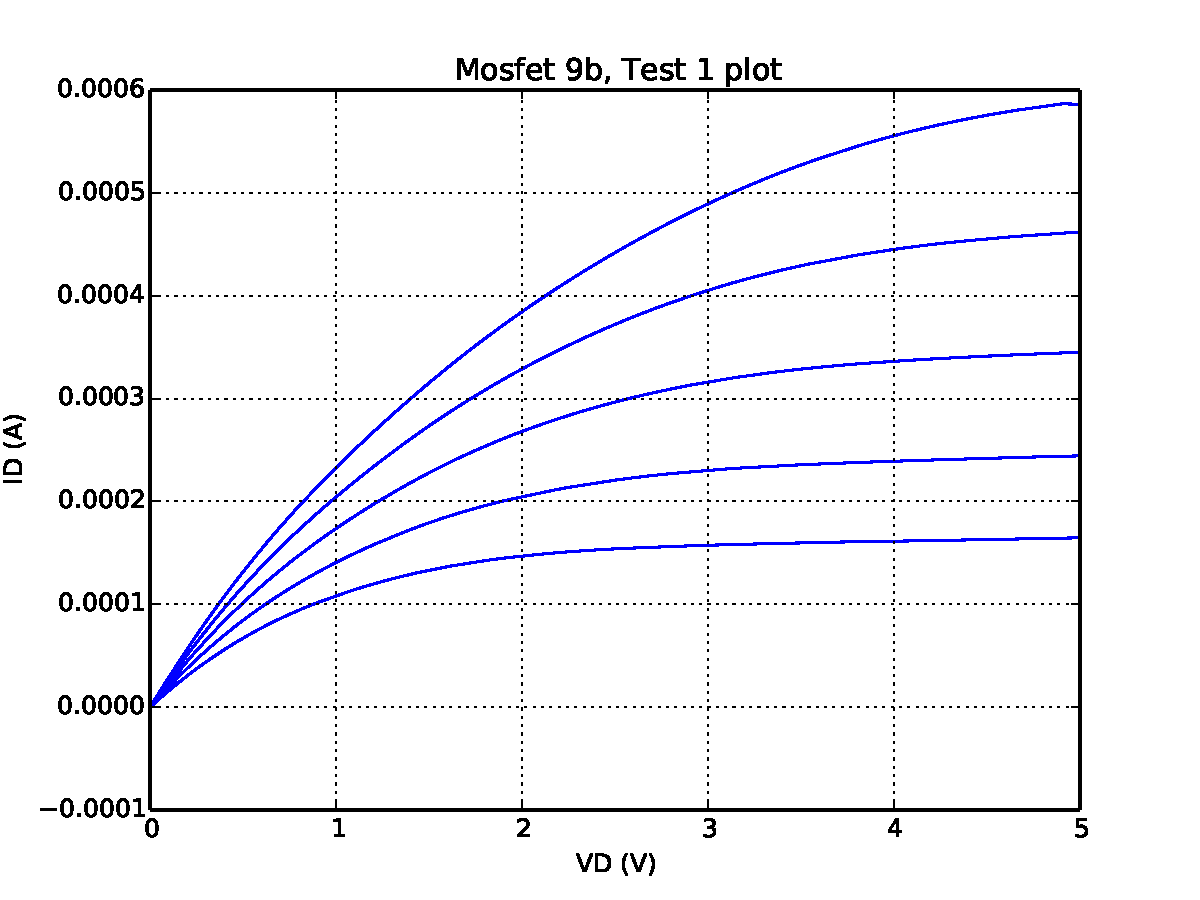
\includegraphics[width=250pt]{Device_plot_data/D9b1plot.pdf}};
\end{tikzpicture}
\caption{Test 1 for Mosfet 9b}
\end{figure}

Calculate stuff here...

\begin{figure}[H]
\centering
\begin{tikzpicture}
\node at (5,5) {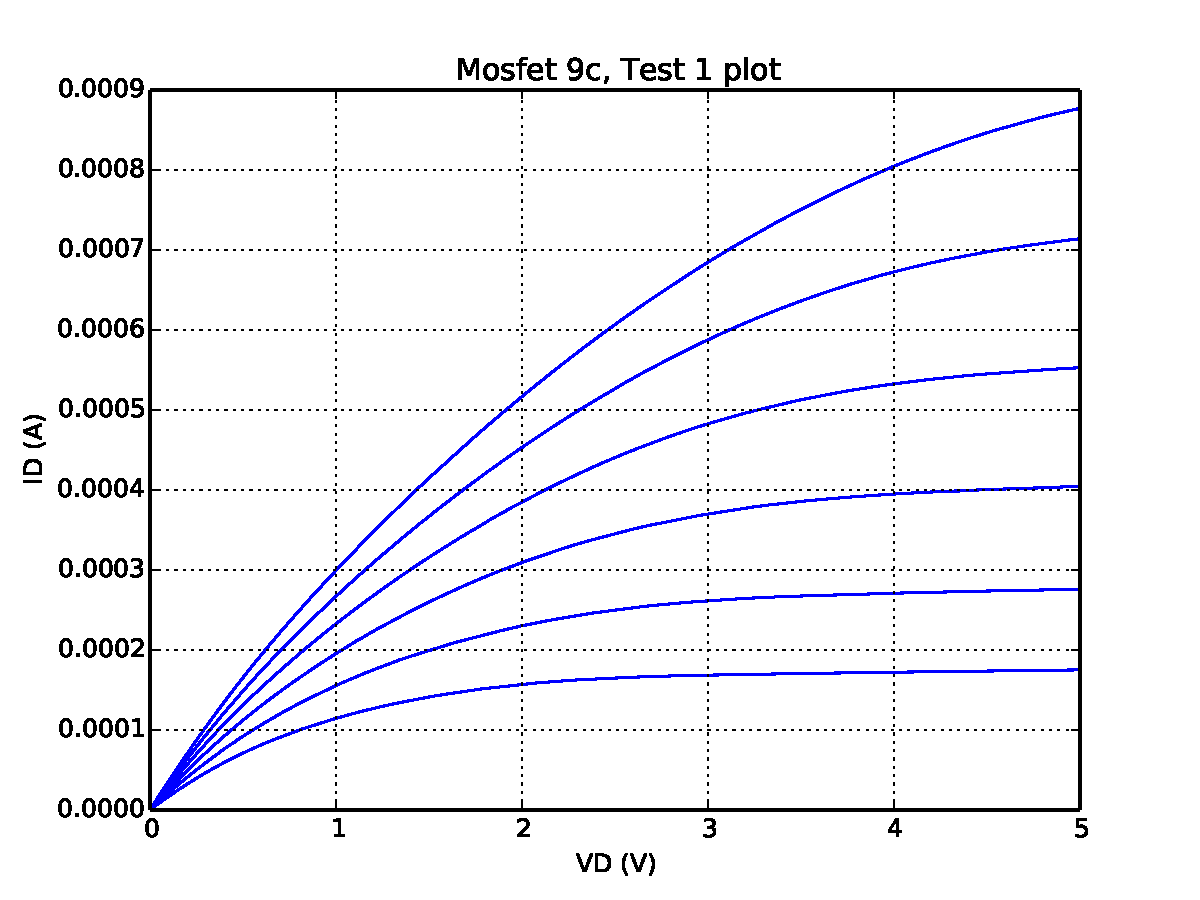
\includegraphics[width=250pt]{Device_plot_data/D9c1plot.pdf}};
\end{tikzpicture}
\caption{Test 1 for Mosfet 9c}
\end{figure}

Calculate stuff here...

\subsubsection{Plots of $I_D$-$V_G$, sweeping $V_B$}

\begin{figure}[H]
\centering
\begin{tikzpicture}
\node at (5,5) {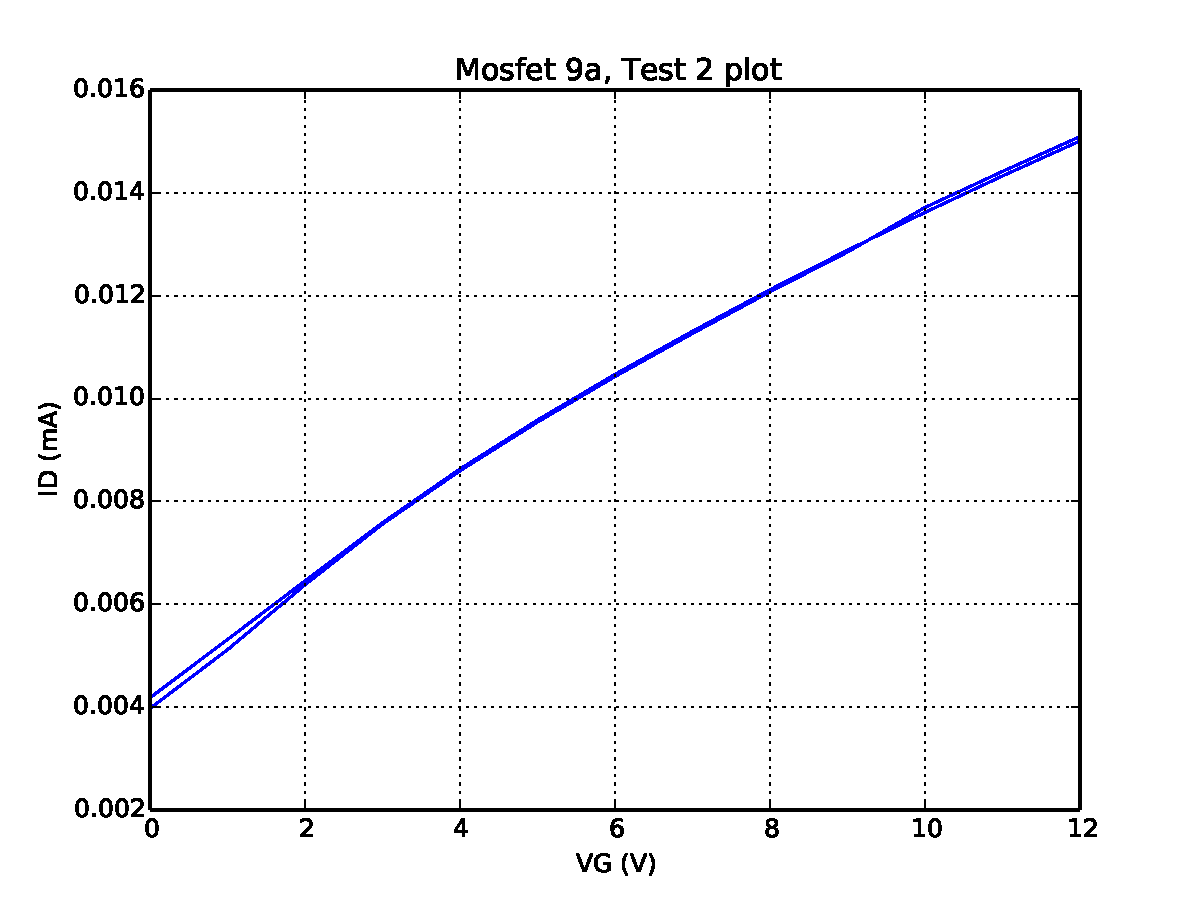
\includegraphics[width=250pt]{Device_plot_data/D9a2plot.pdf}};
\node at (15,5) {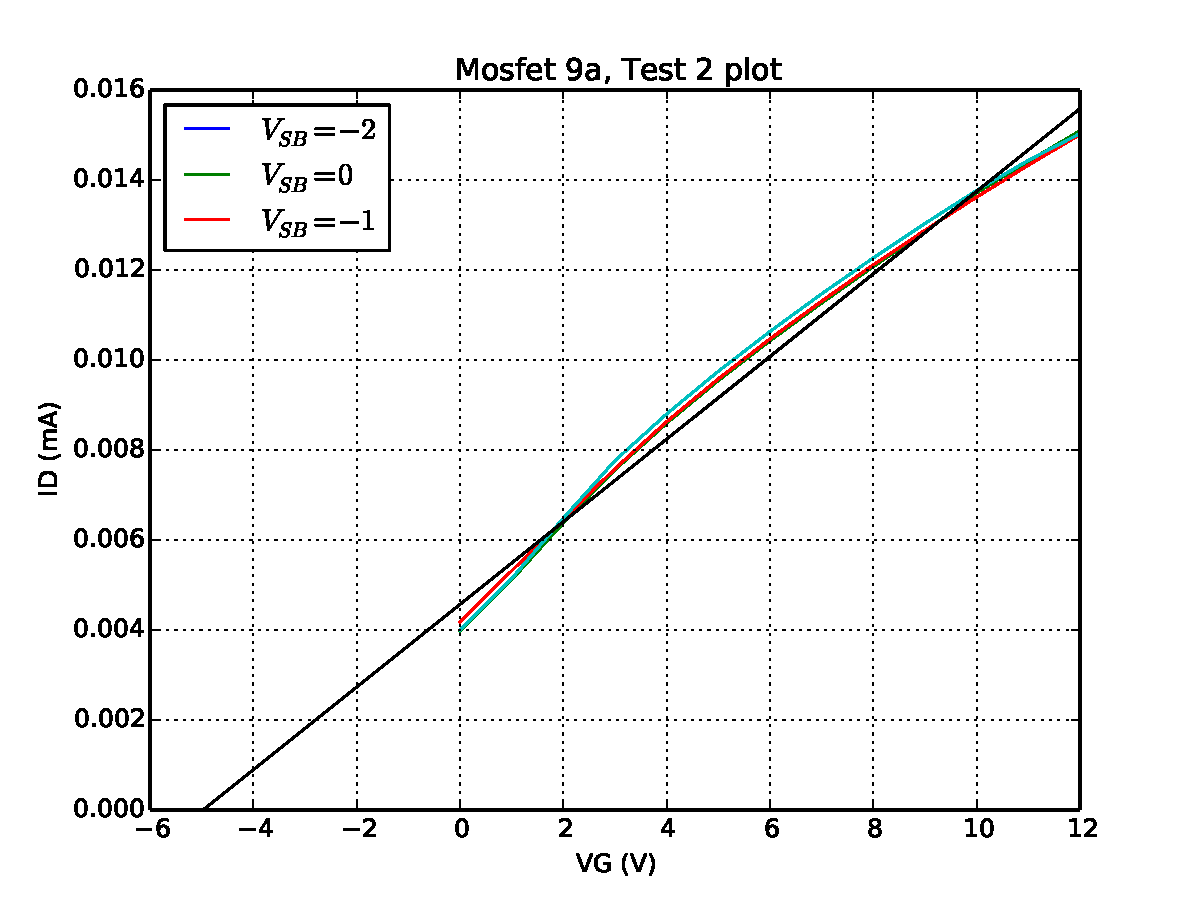
\includegraphics[width=250pt]{Device_plot_data/D9a2linplot.pdf}};
\end{tikzpicture}
\caption{Test 2 for Mosfet 9a. On the right side we did a linear regression on the $V_{\text{SB}} = 0$ line in order to get a estimate of the threshold voltage.}
\label{fig:9alin}
\end{figure}

Using linear regression, we calculated a threshold voltage of $V_t = -4.98$.

\begin{figure}[H]
\centering
\begin{tikzpicture}
\node at (5,5) {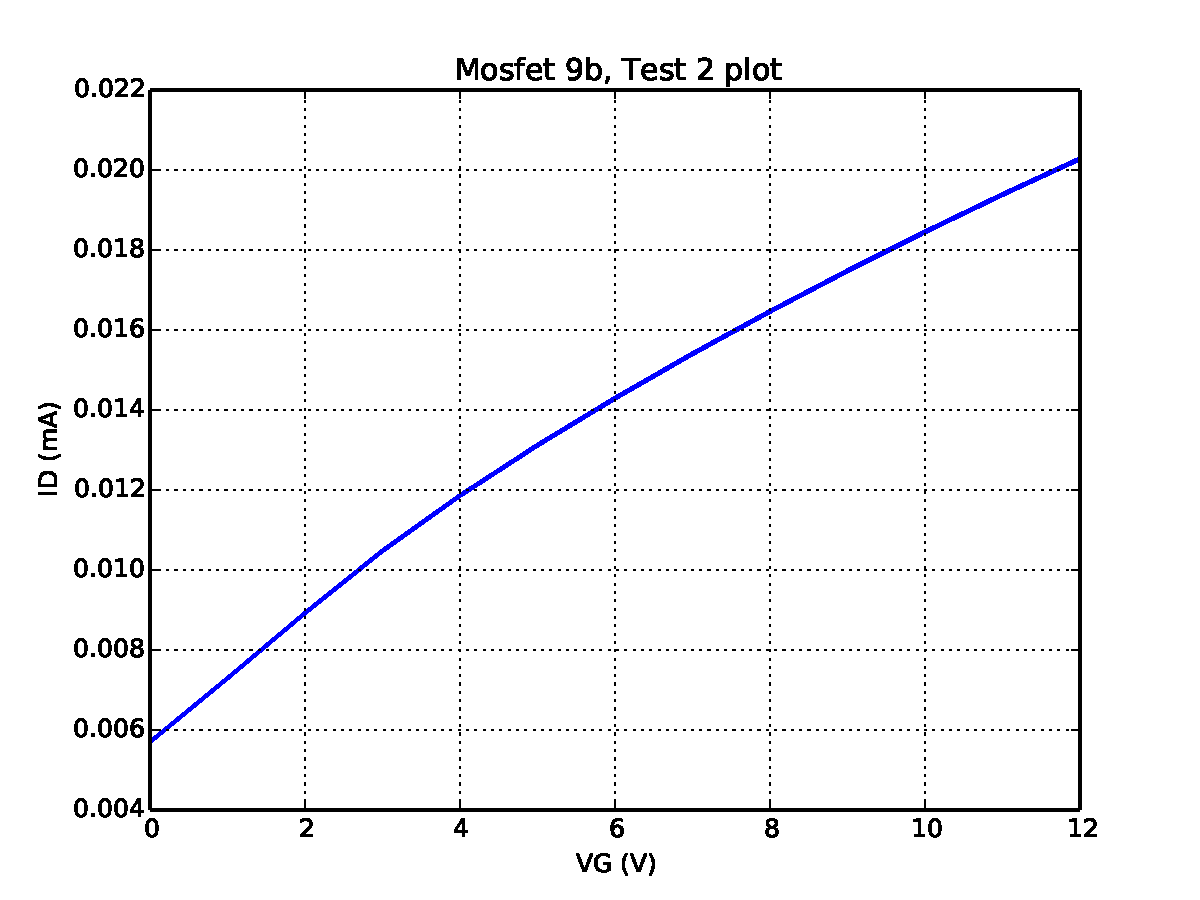
\includegraphics[width=250pt]{Device_plot_data/D9b2plot.pdf}};
\node at (15,5) {\includegraphics[width=250pt]{Device_plot_data/D9b2linplot.pdf}};
\end{tikzpicture}
\caption{Test 2 for Mosfet 9b. On the right side we did a linear regression on the $V_{\text{SB}} = 0$ line in order to get a estimate of the threshold voltage.}
\label{fig:9blin}
\end{figure}

Using linear regression, we calculated a threshold voltage of $V_t = -5.46$.

\begin{figure}[H]
\centering
\begin{tikzpicture}
\node at (5,5) {\includegraphics[width=250pt]{Device_plot_data/D9c2plot.pdf}};
\node at (15,5) {\includegraphics[width=250pt]{Device_plot_data/D9c2linplot.pdf}};
\end{tikzpicture}
\caption{Test 2 for Mosfet 9c. On the right side we did a linear regression on the $V_{\text{SB}} = 0$ line in order to get a estimate of the threshold voltage.}
\label{fig:9clin}
\end{figure}

Using linear regression, we calculated a threshold voltage of $V_t = -4.91$.

\subsubsection{W calculation and plot}
To summarize the threshold voltages calculated in the last section,
\begin{figure}[H]
\centering
\begin{tabular}{c || c | c | c }
MOSFET device & $V_t (V)$ & $W_{\text{drawn}}$ ($\mu m$) & Fig \# \\ \hline
9a & -4.98 & 10 & \textcolor{blue}{\ref{fig:9alin}} \\ \hline
9b & -5.46 & 15 & \textcolor{blue}{\ref{fig:9blin}}\\ \hline
9c & -4.91 & 20 & \textcolor{blue}{\ref{fig:9clin}}\\ \hline
\end{tabular}
\caption{Threshold voltages for all MOSFET 8 devices.}
\label{tab:wdata}
\end{figure}

Now to calculate the channel width we first plot the reciprocal of the measured resistance vs channel width (from lecture).
\begin{figure}[H]
\centering
\begin{tikzpicture}
\node at (5,5) {\includegraphics[width=250pt]{Device_plot_data/D9Rplot.pdf}};
\draw[<-,red] (2,2.1) -- (2,1.8);
\draw[<-,red] (3.65,2.1) -- (3.65,1.8);
\draw[-,red] (2,1.8) -- (3.65,1.8);
\draw[->,red] (2.8,1.8) -- (2.8,1.5);
\node at (2.8,1.3) {$\Delta W$};
\end{tikzpicture}
\caption{1/R vs the channel Width. A linear regression was used to fit the data points. Note that it intersects zero at a negative length.}
\end{figure}

The line above intercepts the x axis at -8.33 $\mu $. Hense our $\Delta W = -8.33\mu m$. Now to plot the threshold voltage vs the efffective channel width we can use Figure \textcolor{blue}{\ref{tab:wdata}}. Note that $W_{\text{eff}} = W_{\text{drawn}} - \Delta W$.

\begin{figure}[H]
\centering
\begin{tikzpicture}
\node at (5,5) {\includegraphics[width=250pt]{Device_plot_data/D9Wplot.pdf}};
\end{tikzpicture}
\caption{Channel threshold voltage vs the channel width. Note the odd V shape which appears because of the calculated threshold voltages.}
\end{figure}

\subsection{Large MOSFET, 10} %%%%%%%%%%% LARGE MOSFET 10

\subsubsection{Measurement setup}
\begin{figure}[H]
\centering
\begin{tikzpicture}

\node at (5,5) {\includegraphics[width=200pt]{Device_setup/device10a2.pdf}};
\node at (15,5) {\includegraphics[width=200pt]{Device_setup/device10a2.pdf}};
\node at (5,9) {\textbf{Test 1}};
\node at (15,9) {\textbf{Test 2}};
\node at (3.5,6) {\textbf{D}};
\node at (7,6) {\textbf{S}};
\node at (4.3,3.5) {\textbf{G}};
\draw[<->,thick] (3,5) -- (3,2.3); % Drain
\node at (3.5,1.9) {V sweep, 0 to 5 V, measure I, V};
\draw[<->,thick] (7.1,5.5) -- (8,7.3); % source
\node at (8,7.5) {constant};
\draw[<->,thick] (5.5,3) -- (8,3) -- (8,3.3); % Gate
\node at (8.5,3.6) {V sweep, 0 to 5 V, step size 1};
\node at (5,8.5) {Stage connector is GND}; % Stage connector, B
%%%%
\node at (15,8.5) {Stage connector V sweep, 0 to -2 V, step size 2};
\draw[<->,thick] (12.4,4.9) -- (11.5,6.4); % Drain
\node at (11,6.5) {Constant, comp 0.05, measure I};
\draw[<->,thick] (17.5,5) -- (17.5,3.7);
\node at (17.6,3.5) {Constant};
\draw[<->,thick] (15,3) -- (15,2) -- (11,2) -- (11,2.5);
\node at (11.5,3) {V sweep, 0 to 12 V, measure V};
\end{tikzpicture}
\caption{Measurement setup for Mosfet 10. This mosfet has very large dimensions compared to others.}
\end{figure}

\subsubsection{Plots of $I_D$-$V_D$, sweeping $V_G$ }
\begin{figure}[H]
\centering
\begin{tikzpicture}
\node at (5,5) {\includegraphics[width=250pt]{Device_plot_data/D101plot.pdf}};
\end{tikzpicture}
\caption{Test 1 for Mosfet 10}
\end{figure}

\subsubsection{Plots of $I_D$-$V_G$, sweeping $V_B$}

\begin{figure}[H]
\centering
\begin{tikzpicture}
\node at (5,5) {\includegraphics[width=250pt]{Device_plot_data/D102plot.pdf}};
\node at (15,5) {\includegraphics[width=250pt]{Device_plot_data/D102linplot.pdf}};
\end{tikzpicture}
\caption{Test 2 for Mosfet 10. On the right side we did a linear regression on the $V_{\text{SB}} = 0$ line in order to get a estimate of the threshold voltage.}
\end{figure}

The threshold voltage here is $V_t = -4.92 V$.

\subsubsection{Calculating mobility, threshold, and other parameters}
To calculate the effective electron mobility we will use the following equation,
\begin{equation}
\mu_{\text{eff}}(V_G) = \frac{I_D}{\frac{W_{\text{eff}}}{L_{\text{eff}}}C_{\text{gox}}(V_{GS} - V_t)V_{DS}}
\end{equation}
Note that $I_D$ depends on $V_{G}$ from the previous plot. For $\Delta W$ and $\Delta L$ we will use values calculated earlier (-8.33 and 1.59 $\mu m$). MOSFET 10 has a W and L value of 100 $\mu m$. Threshold voltage was calculated as $V_t = -4.92 V$ and $V_{DS} = 0.05 V$. $C_{\text{gox}}$ was also calculated earlier as 1.95pF/${\mu\text{m}}^{2}$.
\begin{align*}
\mu_{\text{eff}}(V_G) = \frac{I_D}{\frac{W_{\text{eff}}}{L_{\text{eff}}}C_{\text{gox}}(V_{GS} - V_t)V_{DS}} = \frac{I_D(V_G)}{\frac{(100 + 8.33)\e{-6}}{(100 - 1.59)\e{-6}}(1.95\e{-4}\text{cm}^{-2})(V_{GS} + 4.92)(0.05)} = \frac{I_D(V_G)}{1.07\e{-5}(V_{GS} + 4.92)}{\text{cm}}^2/\text{V-s}
\end{align*}

Now we plot $\mu_{\text{eff}}(V_G)$ vs $V_G$ using the values for $I_D(V_G)$ from the previous graph (Figure 44).
\begin{figure}[H]
\centering
\begin{tikzpicture}
\node at (5,5) {\includegraphics[width=250pt]{Device_plot_data/D10Uplot.pdf}};
\end{tikzpicture}
\caption{Note how the graph levels off almost immediately. The first few data points are right above the threshold voltage.}
\end{figure}

Now if we do a linear fit to each line in Figure 44 we get the following results,

\begin{figure}[H]
\centering
\begin{tabular}{c || c}
$V_{SB}$ (V) & $V_t$ (V) \\ \hline
0 & -4.92 \\ \hline
1 & -4.55 \\ \hline
2 & -4.18 \\ \hline
\end{tabular}
\caption{Results from doing a linear fit to each line in Figure 44 above.}
\end{figure}

With this data we can now make a $V_t(V_{SB})$ vs $\sqrt{V_{SB} + 0.7}$ plot in order to estimate our body effect parameter $\gamma$.
\begin{figure}[H]
\centering
\begin{tikzpicture}
\node at (5,5) {\includegraphics[width=250pt]{Device_plot_data/D10Gplot.pdf}};
\end{tikzpicture}
\caption{The slope of the above plot is our body effect parameter}
\end{figure}
Since we only have 3 data points for $V_{SB}$ our plot is not very accurate and does not show the change of slope as would be present in the theoretical case. Nonetheless, the slope for the above plot is$\gamma$ = 0.910. The equation for $\gamma$, the body effect parameter, is:
\begin{equation}
\gamma = \frac{\sqrt{2\epsilon_{\text{si}} q N_A}}{C_{\text{gox}}} = 
\end{equation}
Solving for the surface concentration and using previous values of $C_{\text{gox}} = 0.195 $mF/${\text{cm}}^2$.
\begin{align*}
N_A = \frac{(\gamma C_{\text{gox}})^2}{2q\epsilon_{\text{si}}} = \frac{(0.910*0.195\e{-3})^2}{2(1.602\e{-19})(11.7\times 8.85\e{-12})} = 9.49\e{20} {\text{cm}}^{-3}
\end{align*}
Finally, we plot a log plot of the data in Figure 44.
\begin{figure}[H]
\centering
\begin{tikzpicture}
\node at (5,5) {\includegraphics[width=250pt]{Device_plot_data/D102logplot.pdf}};
\end{tikzpicture}
\caption{Log plot of Figure 44.}
\end{figure}
The subthreshold slope was calculate between $V_G = 0$ and $V_G = 1$. This slope was calculated to be 0.12 $(V^{-1})$.


\subsection{Inverter, 14} %%%%%%%%%%%%% Inverter 14

\subsubsection{Measurement setup}
\begin{figure}[H]
\centering
\begin{tikzpicture}
\node at (5,5) {\includegraphics[width=350pt]{Device_setup/device14a2.pdf}};
\node at (4.7,6.2) {\textbf{D}};
\node at (4.7,3) {\textbf{S}};
\node at (1.2,4) {\textbf{G}};
\node at (6.6,5) {\textbf{B}};
\draw[<->,thick] (4.8,6.4) -- (6,7); %Drain
\node at (6,7.2) {V sweep, 5 to 15 V, step 5 V};
\draw[<->,thick] (4.7,2.7) -- (4.7,1.5); %Source
\node at (4.7,1.3) {Constant (GND)};
\draw[<->,thick] (6.8,5) -- (7.8,5); %Base
\node at (9.5,5) {Constant, measure V};
\draw[<->,thick] (1.0,4) -- (0,3); %Gate
\node at (-1,2.7) {V sweep, -5 to 5 V, measure V};
\end{tikzpicture}
\caption{Setup for the inverter. Note that the source is connected to a GND and not the stage connector.}
\end{figure}

\subsubsection{b. $V_{\text{in}}-V_{\text{out}}$ plot}
\begin{figure}[H]
\centering
\begin{tikzpicture}
\node at (5,5) {\includegraphics[width=250pt]{Device_plot_data/D14plot.pdf}};
\end{tikzpicture}
\caption{Plot for Inverter. Note both axis are in units of Volts.}
\end{figure}

To find the point where $V_{IN}$ = $V_{OUT}$ we ran a simple loop to find the closest point. We calculated $V_M = 0.025 V$. At that voltage $|V_{OUT} - V_{IN}|$ is minimized.

\section{Theoretical Calculations}

\subsection{Measured Physical Dimensions and Parameters}

\begin{figure}[H]
\centering
\begin{tabular}{c || c}
Parameter & Measured Value \\ \hline
Field $t_{\text{ox}}$ & 477.2 nm \\ \hline
Gate $t_{\text{ox}}$ & 86.5 nm \\ \hline
Intermediate $t_{\text{ox}}$ & 320 nm \\ \hline
$X_j$ & 1000 nm \\ \hline
$X_{j\text{,lateral}}$ & 880 nm \\ \hline
$N_D$ & $10^{21}\,\text{cm}^{-3}$ \\ \hline
\end{tabular}
\end{figure}

\subsection{Resistors [2a,2b]}
According to the results from Lab 1, we had a junction depth of 1$\mu$m and a surface concentration of $10^{21}{\text{cm}}^3$. Using Irvin’s curves  (Fig 4.16(b) in Jaeger), we determined a theoretical sheet resistance of $R_s \approx 10 \Omega$/sq. for the sheet resistance of the active layer (device 2a).

Due to the polysilicon deposition having been performed in NanoLab, we did not have access to the sheet resistance of the polysilicon layer. According to [2], n+ polysilicon sheet resistance for a 500nm layer is 20 $\Omega$/sq. Then, for a layer of 400nm, the sheet resistance of the polysilicon (device 2b) should be 25 $\Omega$/sq.
\begin{align*}
R_{400}=R_{500}\frac{t_{500}}{t_{400}} =20\Omega/sq.\frac{500\text{nm}}{400\text{nm}} = 25 \Omega/sq.
\end{align*}

\subsection{Contact Resistances [17a,17b]}
Sintering of the contacts was performed at 400$\degree$C. Theoretical contact resistivties were taken from Jaeger Fig. 7.6. For device 17a, metal on n+polySi over n-Si should give a 5.6\e{-5} $\Omega$-$\text{cm}^2$ resistivity. For device 17b, metal on n+Si should give a 4.4\e{-4} $\Omega$-$\text{cm}^2$ resistivity. 
\begin{align*}
R=\frac{\rho_c}{A} =\frac{\rho_c}{(5\e{-4}\text{cm})^2}
\end{align*}
So, for device 17a, a contact resistance of 224 $\Omega$ would be expected. For device 17b, a contact resistance of 1760 $\Omega$ would be expected. 


\subsection{Contact-Chain Resistors [2c, 2d]}
\subsubsection{Diffusion chain resistor, 2c}
$R_c$ is the contact resistance calculated earlier and $R_s$ is the sheet resistance calculate for the diffused resistor. $\eta$ is a geometrical constant that has a value of 2.3
\begin{align*}
R_{\text{total}} = 7(\eta R_s + R_c) = 7((2.3)(10) + (1760)) = 12.5k\Omega
\end{align*}
\subsubsection{Poly chain resistor, 2d}
$R_c$ is the contact resistance calculated earlier and $R_s$ is the sheet resistance calculate for the poly resistor. $\eta$ is a geometrical constant that has a value of 2.3
\begin{align*}
R_{\text{total}} = 7(\eta R_s + R_c) = 7((2.3)(25) + (224)) = 1.97k\Omega
\end{align*}


\subsection{Gate/Field Oxide Capacitors[3,4]}

\begin{description}[style = nextline]
\item[Describe the physics of the MOS capacitor. In particular, what does MOS mean? Discuss the three regions of an MOS capacitor.] 

MOS stands for metal-oxide-semiconductor: the three components that form a MOS capacitor. One plate is formed by the metal (or polysilicon) gate, and the other is formed by the surface of a semiconductor, with a oxide layer as an insulator in between. MOS capacitators have three operating regions due to the nature of the semiconductor. In the accumulation region, the applied gate voltage is lower than the flatband voltage of the device. Negative charge accumulating on the gate attracts holes from the p-substrate. In the depletion region, the gate voltage increases beyond the flatband voltage. Positive charge accumulates on the gate, repelling positive holes in the p-substrate, creating a depletion region in the semiconductor. In the inversion region, the gate voltage increases beyond the threshold voltage, and minority carriers, in this case electrons, in the p-substrate are attracted to the surface of the substrate by the large amount of positive charge on the gate.

\item[Why does the Intermediate Oxide Capacitor (5) not display MOS effects?] 

Due to the fact that the intermediate oxide was grown during drive-in for the S/D regions, there is an exceedingly large amount of dopants in the intermediate oxide, as opposed to the gate and field oxide which were grown when the wafer had not been heavily doped. If these are included into the calculations, then both the flatband voltage and the threshold voltage are exceedingly negative and the capacitor remains permanently in the accumulation region and never transitions.for the given voltage range.
\end{description}

\subsubsection{Theoretical plots}
\begin{figure}[H]
\centering
\begin{tikzpicture}
\node at (5,4) {CV plot for \textcolor{blue}{Gate capacitance} and \textcolor{red}{Field capacitance}};
\draw[<->,thick] (0,0) -- (10,0);
\draw[->,thick] (5,0) -- (5,2.5);
\node at (10.2,0) {$V_G$};
\node at (5.2,2.7) {$C_G$};

\draw[-,dashed,red] (2.5,0) -- (2.5,2.5);
\draw[-,dashed,blue] (2.83,0) -- (2.83,2.5);
\draw[-,dashed,blue] (5.5,0) -- (5.5,2.5);
\draw[-,dashed,red] (9,0) -- (9,2.5);
\node at (2.5,-0.5) {\textcolor{blue}{$V_{FB}$ = -0.95V}};
\node at (2.5,-1) {\textcolor{red}{$V_{FB}$ = -0.84V}};
\node at (5.5,-0.5) {\textcolor{blue}{$V_t$ = 0.03V}};
\node at (9,-0.5) {\textcolor{red}{$V_{t}$ = 1.30V}};

\draw[red] (2,2.5) -- (2.5,2.5) parabola bend (8,0.5) (8.5,0.5) parabola bend (8.5,0.5) (9.5,2.5) -- (10,2.5);
\draw[blue] (2.6,2.5) -- (2.83,2.5) parabola bend (4.8,0.5) (5,0.5) parabola bend (5,0.5) (6,2.5) -- (7,2.5);

\end{tikzpicture}
\caption{}
\end{figure}



\subsubsection{Theoretical calculations}
Assuming no fixed charge in the oxide and oxide/silicon interface, the flatband voltage is the work function of the capacitor given by the equation:
\begin{equation}
V_{FB} = \Phi_M - \chi - E_g/2q - |\Phi_F|
\end{equation}
Where
\begin{equation}
|\Phi_F| = \frac{kT}{q}\ln{N_B/n_i}
\end{equation}
For gate oxide $\Phi_M - chi = 0$, $E_g$ = 1.12eV, and $N_B$ is the background concentration of the wafer.
\begin{align*}
|\Phi_F| =& \frac{kT}{q}\ln{N_B/n_i} = \frac{1.38\e{-23}298}{1.602\e{-19}}ln{8\e{14}/10^{10}} = 0.28V \\
V_{FB} =& \Phi_M - \chi - E_g/2q - |\Phi_F| = 0 - (1.12eV)/(2*1.602\e{-19}) - 0.28 = -0.84
\end{align*}
For Field oxide $\Phi_M - chi = -0.11$, $E_g$ = 1.12eV. This means $\Phi_F = 0.28$ which is the same value as before.
\begin{align*}
V_{FB} =& \Phi_M - \chi - E_g/2q - |\Phi_F| = -0.11 - (1.12eV)/(2*1.602\e{-19}) - 0.28 = -0.84 = -0.95
\end{align*} 
Again, assuming no fixed charge in the oxide and oxide/silicon interface, the threshold voltage is given by the equation:
\begin{equation}
V_{TN} = V_{FB} + 2|\Phi_F| + (1/C_0)\sqrt{4 \epsilon_s q N_B |\Phi_F|}
\end{equation}
$V_{FB}$ and $|\Phi_F|$ are defined above. $C_0 =\epsilon_{ox}/t_{ox} = (3.9\times8.85\e{-12})/(86.5\e{-9}) = 3.99\e{-4}$ F/m.
\begin{align*}
V_{TN} =& V_{FB} + 2|\Phi_F| + (1/C_0)\sqrt{4 \epsilon_s q N_B |\Phi_F|} \\
=& -0.84 + 2(0.28) + (1/3.99\e{-4})\sqrt{4(11.7\times 8.85\e{-12})1.602\e{-19}(8\e{14})0.28} = 0.03 V
\end{align*}
For the field oxide $C_0 =\epsilon_{ox}/t_{ox} = (3.9\times8.85\e{-12})/(477.2\e{-9}) = 7.22\e{-5}$ F/m.
\begin{align*}
V_{TN} =& V_{FB} + 2|\Phi_F| + (1/C_0)\sqrt{4 \epsilon_s q N_B |\Phi_F|} \\
=& -0.95 + 2(0.28) + (1/7.22\e{-5})\sqrt{4(11.7\times 8.85\e{-12})1.602\e{-19}(8\e{14})0.28} = 1.30 V
\end{align*}
The photoelectric effect will cause carriers to be generated in the semiconducter. This will cause the capacitance to be appear slightly higher when transitioning between the accumulation and inversion regions when measured in ambient light than when measured in the dark.

\subsection{Diode}
We make the assumption that the junction is a step junction and that the concentrations of dopants are constant across respective regions of the device. Built-in potential for a p-n diode is given by the function:
\begin{equation}
\phi = \frac{kT}{q}\ln{\frac{N_AN_d}{{n_i}^{2}}}
\end{equation}
Where T is room temperature, $N_A$ is the p-sub dopant concentration (8\e{14}${\text{cm}^{-3}}$), $N_d$ is the n+ dopant concentration ($10^{21}{\text{cm}^{-3}}$), and $n_i$ is the instrinsic carrier concentration for silicon ($10^{10}$).

\begin{align*}
\phi = \frac{kT}{q}\ln{\frac{N_AN_d}{{n_i}^{2}}} = \frac{1.38\e{-23}(298)}{1.602\e{-19}}\ln{\frac{(8\e{14})(10^{21})}{{10^{20}}}} = 0.92 V
\end{align*}

\subsection{MOSFETs}
\subsubsection{MOSFETs of varying length [8] and width [9]}
\subsubsection{Large MOSFET}

\subsection{Inverter}
\begin{figure}[H]
\centering
\begin{tikzpicture}
\node at (5,5) {\includegraphics[width=350pt]{Device_setup/Inverter_plots.pdf}};
\end{tikzpicture}
\caption{Setup for inverters.}
\end{figure}

\subsubsection{Theoretical Inverter Calculations}

The load resistor has Vdd connected to the drain and the gate. Since
\begin{align*}
V_{DS} &= V_{dd} - V{out} \\
V_{GS} &= V_{dd} - V_{out}
\end{align*} 
Then 
\begin{align*}
V_{DS} = V_{dd} - V_{out} >= V_{dd} - V_{out} - V_{tnl} = V_{GS} - V_{tnl}
\end{align*}
So the load transistor is always in the saturation region, regardless of Vdd. It therefore acts as a variable resistor dependent on Vdd. The threshold voltage for both NMOS transistors is:
\begin{align*}
V_{TN} = V_{FB} + 2|\Phi_F| + (1/C_0)\sqrt{2\epsilon_s q N_B (2|\Phi_F| + V_{sb})}
\end{align*}
They differ in $V_{sb}$ so 
\begin{align*}
V_{tnl} &= V_{TN0} + (1/C_0)\sqrt{2\epsilon_s q N_B}(\sqrt{2|\Phi_F| + V_{out}} - \sqrt{2|\Phi_F|}) \\
V_{tnd} &= V_{TN0} \\
\text{Where } V_{TN0} =& V_{TND} = 0.03
\end{align*}
Since $V_{tnl}$ is dependent on $V_{out}$ and vice versa, $V_{out}$ can only be determined by iteration. For the purposes of graphing, we will make the simplfying assumption that the effect of substrate bias is small, and thus that $V_{tnl}$ can be estimated to be $V_{TN0}$. This is not the case in reality, but should serve the purpose of illustrating the expected curves.

For the drive transistor: In the cutoff region ($V_{in}<V_{tnd}$), no current flows through the driver transistor, therefore the drain currents are zero for both transistors.
\begin{align*}
I_{Dl} = K_L(V_{dd} - V_{out} - V_{tnl})^2 = 0
\end{align*}
Therefore $V_{out} = V_{dd} - V_{tnl}$. In the saturated region ($V_{out} >V_{in}-V_{tnd}>0$), both transistors are saturated. Their drain currents must be equal.
\begin{align*}
I_{dl} =& K_L(V_{dd} - V_{out} - V_{tnl})^2 = K_D(V_{in} - V_{tnd})^2 = I_{Dd} \\
V_{out} =& V_{dd} - V_{tnl} - \sqrt{K_D/K_L}(V_{in} - V_{tnd})
\end{align*}
In the linear region ($V_{in}-V_{tnd}>V_{out} >0$), the driver transistor is in the linear region and the load transistor is in the saturated region. Since their drain currents must again be equal:
\begin{align*}
I_{dl} =& K_L(V_{dd} - V_{out} - V_{tnl})^2 = 2K_D(V_{in} - V_{tnd} - 0.5V_{out})V_{out} = I_{Dd}
\end{align*}
Here the dependence of Vin on Vout is becomes non-linear. 
\begin{align*}
V_{in} = \frac{(K_L/K_D)(V_{dd} - V_{out} - V_{tnl})^2 + V_{out}^2 + V_{tnd}V_{out}}{2V_{out}}
\end{align*}
Also note that for our transistor, the aspect ratio should be
\begin{align*}
\frac{K_D}{K_L} = \frac{W_DL_L}{L_DW_L} = \frac{160*20}{10*10} = 16
\end{align*}
For $V_{tnl}$ and $V_{tnd}$ we will use a value of 0.3 as mentioned above. $V_{dd}$ will range from 0 to 5 volts.

\subsubsection{Theoretical Inverter plot}
\begin{figure}[H]
\centering
\begin{tikzpicture}
\node at (5,5) {\includegraphics[width=350pt]{Device_plot_data/D14theoplot.pdf}};
\end{tikzpicture}
\caption{Theoretical inverter plot.}
\end{figure}


\section{Discussion}


\section{Optional Questions}

\section{Appendix}
%----------------------------------------------------------------------------------------
%	SECTION References
%----------------------------------------------------------------------------------------
\section{References}
\begin{enumerate}
\item Jaeger, Richard. \textit{Introduction to microelectronic fabrication}. New Jersey: Prentice Hall, 2002. Print.
\end{enumerate}

%----------------------------------------------------------------------------------------
%	SECTION 6
%----------------------------------------------------------------------------------------

% Nothing right now

%----------------------------------------------------------------------------------------
%	BIBLIOGRAPHY
%----------------------------------------------------------------------------------------

\bibliographystyle{apalike}

\bibliography{sample}

%----------------------------------------------------------------------------------------


\end{document}

